\documentclass[10pt]{article}

\usepackage[T1]{fontenc}
\usepackage[utf8]{inputenc}
\usepackage{lmodern}
\usepackage[letterpaper,left=0.82in,right=0.82in,top=0.78in,bottom=0.80in]{geometry}
\usepackage{microtype}
\usepackage{amsmath,amssymb,amsthm}
\usepackage{booktabs,longtable,tabularx,array,multirow}
\usepackage[dvipsnames,table]{xcolor}
\usepackage{graphicx}
\graphicspath{{../figures/}{figures/}}
\usepackage{caption}
\usepackage[section]{placeins}
\usepackage{enumitem}
\usepackage{natbib}
\usepackage[hidelinks]{hyperref}
\usepackage{url}

\definecolor{aphfsnavy}{HTML}{142337}
\definecolor{aphfsblue}{HTML}{315A7D}
\definecolor{aphfslight}{HTML}{EAF0F5}
\definecolor{aphfsgreen}{HTML}{2F6B4F}
\definecolor{aphfsamber}{HTML}{8B5A00}

\hypersetup{
  pdftitle={All-Possibility Hierarchical Filtering Simulation (APHFS): A Resource-Bounded Framework from Executable Rules toward Multiscale Biology, Aging, and Rejuvenation Research},
  pdfauthor={Mingyuan Chen},
  pdfsubject={Resource-bounded executable model search with complete finite-grammar accounting},
  pdfkeywords={model search, systems biology, model-class inadequacy, non-identifiability, coarse-graining, quantum cellular automata, fault-tolerant quantum computing, elementary cellular automata, reproducibility}
}

\setlength{\parindent}{0pt}
\setlength{\parskip}{4.4pt}
\linespread{1.10}
\setlength{\emergencystretch}{2em}
\setlist{leftmargin=1.55em,itemsep=2pt,topsep=3pt}
\captionsetup{font=small,labelfont=bf}
\renewcommand{\arraystretch}{1.13}
\newcommand{\classbad}{\texttt{MODEL\_CLASS\_INADEQUATE}}
% Exact machine tokens retained visibly below:
% RETAIN_CLASS MODEL_CLASS_INADEQUATE NOT_CONTRADICTED_BY_LOCKED_AUDIT
% Policy identifiers: fixed_order development_frozen_order adaptive_fidelity exhaustive
\newcommand{\R}{\mathbb{R}}
\newcommand{\E}{\mathbb{E}}
\newtheorem{theorem}{Theorem}
\newtheorem{proposition}{Proposition}
\theoremstyle{definition}
\newtheorem{definition}{Definition}

\makeatletter
\def\ps@aphfs{%
  \def\@oddhead{\hfil\small APHFS: Resource-Bounded Model Search\hfil}%
  \let\@evenhead\@oddhead
  \def\@oddfoot{\hfil\thepage\hfil}%
  \let\@evenfoot\@oddfoot
}
\makeatother

\title{\color{aphfsnavy}\textbf{All-Possibility Hierarchical Filtering Simulation (APHFS):\\
A Resource-Bounded Framework from Executable Rules\\
toward Multiscale Biology, Aging, and\\
Rejuvenation Research}}
\author{\textbf{Mingyuan Chen}\\
\small Department of Biochemistry and Molecular Biology, Johns Hopkins Bloomberg School of Public Health,\\
\small Johns Hopkins University, Baltimore, Maryland, USA\\
\small Correspondence: \href{mailto:a515006420@gmail.com}{\texttt{a515006420@gmail.com}}}
\date{3 September 2026}

\begin{document}
\pagestyle{aphfs}
\maketitle
\thispagestyle{plain}

\begin{abstract}
Scientific models begin as imagined explanations; mathematics makes them executable, whereas
evidence determines which remain tenable. All-Possibility Hierarchical Filtering Simulation
(APHFS) joins bottom-up candidate generation to top-down reality constraints. ``All'' is local:
within a declared finite grammar, resource envelope, and precision policy, every address receives
a terminal account. The framework preserves observational ambiguity, rejects an inadequate class
only under complete simultaneous bounds, and otherwise permits an indeterminate result. It
withholds coarse-graining until specified upper-level observables and decisions remain stable
under refinement. Future fault-tolerant quantum computers could enlarge executable dynamics, but
would be an execution substrate rather than evidence.

We evaluated this machinery once in the complete 256-rule elementary-cellular-automaton grammar.
The generating rule and operational signature class were retained in all 64 A1 blocks, although
five blocks retained two rules and three retained two classes. A deliberately distinguishable
radius-two construction returned model-class inadequacy in all 64 B1 blocks. D2-CERT used the
provably density-preserving periodic Rule 170 shift: 0/64 calibration and 0/64 held-out violations
checked certificate-pipeline conformance for a constructed closed map, not uncertain coarse-law
accuracy. Four resource policies reached identical decisions. One prespecified salted
pseudo-random early-stopping order was least costly on this constructed workload (75,080 units),
versus 89,816 for the other order, 92,592 for adaptive fidelity, and 132,096 for exhaustive search.

These results establish bounded, failure-capable behavior only for this synthetic finite grammar,
not physical or biological validation. A separately prespecified enzyme-kinetics study is the
next empirical bridge toward multiscale biology; aging and safety-constrained rejuvenation remain
longer-term destinations.
\end{abstract}

\section{Introduction}

Model discovery faces a problem that extends beyond search accuracy. A procedure may find the
best model it was allowed to consider while the whole language is wrong; sparse observations may
support several mechanisms; and a numerical approximation may preserve low-level values yet alter
the upper-level conclusion. A credible search method must expose all three possibilities.

Imagine a person ten thousand years ago who sees the round Sun and proposes that Earth might also
be round, only to be mocked by companions. The round Sun does not prove a spherical Earth, and
ridicule does not refute it. The episode serves one purpose here: to separate hypothesis
generation from evidential validation. An imagined rule must first be expressed precisely enough
to generate consequences and then confronted with observations independent of its formulation.

\paragraph{Core thesis.}
APHFS connects imagination, executable mathematics, and evidence through a resource-bounded
sequence of decisions. Bottom-up generation explores a declared language; top-down observations
constrain each bridge toward higher-level descriptions. Within a fixed finite grammar, resource
envelope, and precision policy, every executable candidate is enumerated or explicitly accounted
for. Observationally equivalent candidates remain ambiguous, a valid simultaneous test may find
the entire class inadequate, and missing support produces an indeterminate result rather than a
convenient conclusion. Coarse-graining is not accepted before its domain, memory, and error
conditions are checked. Lower-level fidelity is sufficient only when prespecified refinements
preserve registered upper-level observables and decisions. Computation can expand what is
evaluated; evidence constrains what can be justified. A future fault-tolerant quantum execution
layer could make some quantum-native candidate dynamics tractable, while adding explicit
state-preparation, error-correction, measurement, and classical-post-processing obligations. It
would not relax complete accounting or turn computation into empirical support. Biology, aging,
and rejuvenation remain downstream empirical destinations.

The motivating intuition is conditional rather than ontological: if progressively expanded
candidate languages are sufficiently expressive for the registered observables, generation and
search reach relevant candidates, independent evidence is sufficiently discriminating, and
estimation, numerical, dynamical, and coarse-graining errors are controlled, then the retained set
may approach the lowest observable risk attainable within the declared comparison envelope. This
does not guarantee recovery of nature's ontology. A grammar may omit the relevant mechanism,
finite observations may retain a set, an entire class may be inadequate, and each new domain
requires new evidence.

The phrase \emph{All-Possibility} is therefore local. It means complete accounting within a stated
grammar, encoding, bit budget, resource envelope, and precision policy---not enumeration of every
law or ontology in nature. Enlarging the language creates a new claim. This boundary separates a
finite scientific object that can be audited from an unrestricted metaphysical assertion.

The framework also separates questions that leaderboards merge. Candidate ranking asks which
member fits best. Operational signatures ask which members the observation interface can
distinguish. A class-level gate asks whether even the best-supported class is inadequate. If a
candidate, bound, or error-budget entry is missing, the class decision is \texttt{INDETERMINATE};
absence is never imputed as evidence against the class.

The long-term destination is biological. The proposed route starts with executable rules below
fixed particle labels and advances only through empirical bridges to physical, chemical,
molecular, and cellular organization. Particle-like candidates must face physical and scattering
constraints; atom-like candidates must face atomic spectra; and molecule-like candidates must
face molecular structure, energy, and reaction data. Whole-cell studies illustrate both the reach of integrated
mechanistic models and the difficulty of validating emergent predictions
\citep{karr2012,thornburg2022,thornburg2026,thornburg2026correction}. Aging would enter when a model
can predict long-horizon homeostatic drift and declining resilience under appropriate longitudinal
and perturbational data \citep{lopezotin2013,lopezotin2023}. Rejuvenation research would require
causal interventions with efficacy, persistence, toxicity, off-target effects, uncontrolled
proliferation, and cancer risk
made explicit. These are downstream research goals, not interpretations of cellular automata.

Here, \emph{pre-particle} is a modeling stance, not an empirical claim of a newly discovered
subparticle ontology. Candidate rules may precede fixed particle labels in the generative
description, but particle-like status must be earned through stable observables and independently
specified physical constraints. Quantum cellular automata are an important future candidate
family, not a conclusion forced by the current ECA study.

Beyond the finite ECA demonstration, candidate languages may vary dimension, geometry, locality,
symmetry, interaction rules, motion, stochasticity, composition, and response to perturbation.
When a declared finite grammar is affordable, APHFS requires genuine enumeration and complete
terminal accounting. When it is not, stratified, randomized, sampled, or adaptive generation may
be used only with its coverage frame and missing mass stated; such a search is not relabeled as
local-All enumeration.

This paper integrates six capabilities needed for such model search: advance definition of the
candidate language, complete accounting, ambiguity-preserving signatures, a whole-class
inadequacy gate, observable-level error and fidelity controls, and a one-time held-out evaluation.
Systems biology provides the motivating decision structure because it must compare mechanistic
explanations under partial observation, misspecification, coarse-graining, and finite compute. The
current experiment uses all 256 elementary cellular automata (ECA) as an inspectable testbed in
which every candidate can receive a terminal account. It evaluates the machinery, not biology.

\section{The APHFS research program}
\label{sec:program}

Figure~\ref{fig:research-ladder} places the current experiment inside the larger research program.
Candidate construction proceeds bottom-up, beginning with executable rules rather than assuming
the higher-level objects it ultimately seeks to explain. Constraints enter top-down as empirical
anchors. Each transition---to persistent structures, particle-like signatures, molecular systems,
cellular dynamics, aging, or intervention---is a new scientific question that can fail.

\begin{figure}[!t]
\centering
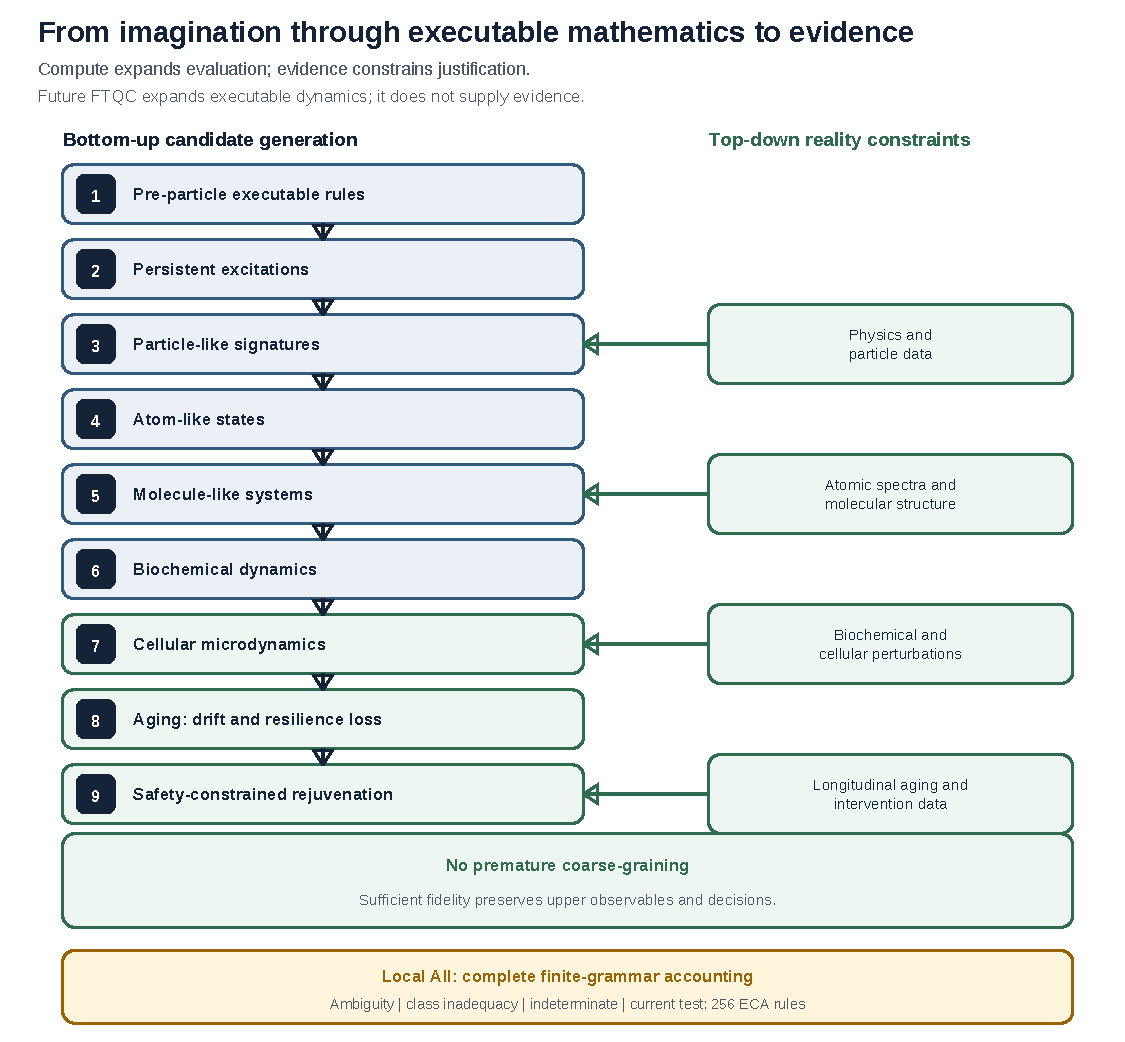
\includegraphics[width=0.90\linewidth]{framework_research_ladder_v3_5.pdf}
\caption{The APHFS research program. Imagination is encoded as executable candidates, complete
finite-grammar accounting makes the search auditable, and empirical constraints determine which
claims survive. Operational ambiguity, model-class inadequacy, and indeterminacy remain distinct.
Higher-level objects require validated coarse-graining and protected upper-observable fidelity.
Future fault-tolerant quantum hardware could expand executable candidate dynamics but would not
supply evidence. The present evidence concerns only the 256-rule ECA machinery test; biology,
aging, and rejuvenation remain downstream destinations.}
\label{fig:research-ladder}
\end{figure}

Two controls govern movement up the ladder. First, a coarse description is accepted only when
its domain, memory, and error conditions support the proposed
upper-level inference. Second, numerical resolution is decision-relative. A fidelity that
preserves water density may not preserve a vibrational spectrum; one that preserves a ball's
center-of-mass trajectory may not preserve surface turbulence. More microscopic precision is
useful only when it can change a registered observable, classification, decision, or certificate.

Aging and rejuvenation therefore occupy the far end of the path. Aging could be represented by
long-horizon distributions of recovery, viable-state return, functional persistence, and entry
into dangerous attractors. Rejuvenation would become a safety-constrained control problem over
combination, order, timing, dose, persistence, and adverse effects, drawing on robust-control
precedents \citep{iyengar2005,nilim2005}. Neither interface is implemented here. Progress depends
on new domain models and observations, not on computational scale alone.

\section{How APHFS works}
\label{sec:six-steps}

The six decisions in Figure~\ref{fig:six-steps} form a dependency chain: each supplies a premise
for the next, and each has a distinct failure meaning.

\begin{figure}[htbp]
\centering
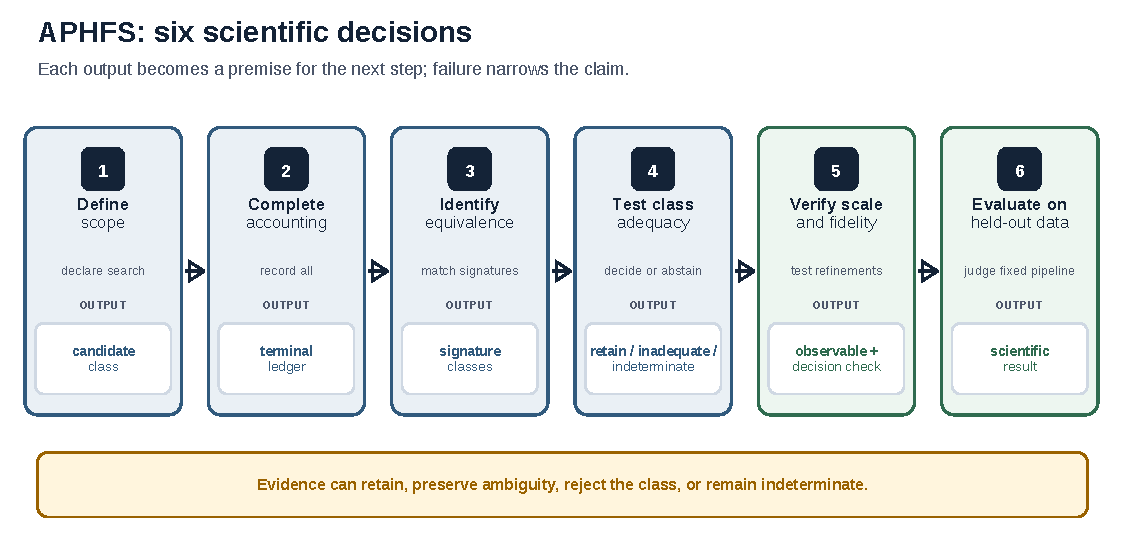
\includegraphics[width=0.94\linewidth]{aphfs_six_step_workflow_v3_5.pdf}
\caption{Six linked decisions in APHFS. Scope precedes complete accounting; operational
equivalence precedes class-adequacy testing; scale and fidelity checks protect the inference; and
held-out evaluation judges the fixed pipeline. Failure narrows the claim, returns an indeterminate
result, or motivates a newly specified study.}
\label{fig:six-steps}
\end{figure}

\subsection{Step 1: Define scope}

The address alphabet, finite address set, single-valued parser, execution semantics, invalid-state
rules, resources, precision policy, probes, and failure actions are fixed before evaluation. This
turns an open-ended idea into a finite scientific object and reveals its expressive limits.
Ledger identity is the declared address (or a predeclared canonical address), so syntactic aliases
remain separate rows unless canonicalization was fixed in advance. Post-outcome changes create a
new study; they cannot expand the old completeness claim.

The declaration therefore answers two questions before any ranking begins: which mechanisms are
expressible, and which executions are affordable. Invalid syntax, invalid semantics, and exhausted
resources remain visible outcomes. If a relevant mechanism cannot be represented, the limitation
belongs to the candidate class; retained models do not become exhaustive over nature.

\subsection{Step 2: Complete accounting}

Every addressable candidate must be executed or receive an explicit terminal record, including
invalid syntax, numerical failure, and resource exhaustion. Here all 256 ECA rule IDs were
accounted for. A0 compared rule tables and trajectories under periodic, fixed-zero,
fixed-one, and edge-replicate boundaries (historical code token: \texttt{reflect}); A1 used its
separate block-level interface. The edge-replicate convention sets each out-of-range neighbor to
the nearest boundary cell, rather than reflecting the next interior cell. A0's scalar
reference and NumPy-vectorized production paths were separately implemented within the same
AI-assisted project and do not share their rule-lookup or one-step update functions. Their
agreement is an internal implementation-conformance check, not a separately authored
implementation or external replication.
An absent candidate
breaks whole-class inference. A partial run may still be useful, but its sampling frame must be
stated.

This accounting is the premise for every later statement about the declared class. An unrecorded
timeout or silently imputed failure breaks that premise because an unseen candidate could change
the conclusion. Computational scarcity may narrow the searchable scope; it cannot assign a
favorable value to missing evidence.

\subsection{Step 3: Identify operational equivalence}

Fixed probes and deterministic quantizers map each candidate to a canonical signature. Exact
serialized equality partitions candidates that the observation interface cannot distinguish;
candidate losses remain separate unless equality holds across the full evaluation interface.
The result is set-valued identification, not ontological identity. A changed probe, tolerance, or
serialization rule defines a new partition.

Operational equivalence makes ambiguity measurable. More informative observations may split a
signature class, but an arbitrary representative cannot make the unresolved alternatives
disappear. Equality under finitely many probes therefore supports claims about that interface
alone, not agreement on unseen inputs or a unique underlying mechanism.

\subsection{Step 4: Test class adequacy}

Ranking always produces a least-bad member, so APHFS asks whether simultaneous lower loss bounds
place every candidate above a prespecified threshold. Bounds are formed at candidate level and
aggregated conservatively through signature classes. Whole-class inadequacy is reported only with
complete candidate or class coverage and a complete alpha ledger. A missing run, invalid bound,
unsafe deduplication, or incomplete ledger returns \texttt{INDETERMINATE}, never evidence against
the class.

In the present B0/B1 workload every class was a singleton and every loss was computed on complete
finite support. Thus the class minimum and the general repeated-look allocation were definitions
of the wider framework, not empirically exercised features of these endpoints. The observed B
outcomes test exact-loss decision and completeness machinery for their constructed cases.

A valid inadequacy result has a different consequence from a poor winner: it sends the search back
to the language or resource envelope before further ranking is useful. Conversely, incomplete
uncertainty control requires abstention. The procedure is designed to distinguish a bad model
from a bad language and both from insufficient evidence.

\subsection{Step 5: Verify scale and fidelity}

Trajectory bounds track propagated local error; cross-scale bounds compare evolve-then-coarse-
grain with coarse-grain-then-evolve on declared domains; memory checks test whether a coarse state
supports prediction. Each fidelity record names the lower-level refinement, protected upper-level
observable, tolerance, horizon, input or environment distribution, decision stability, and need
for further refinement. Domain exit, missing output, or an observable or decision breach blocks a
sufficiency claim. Raw datatype agreement is not enough.

The scientific question is not whether two floating-point arrays are numerically close in the
abstract, but whether refinement can change the registered conclusion. Microscopic discrepancies
may contract or amplify, whereas further precision may be unnecessary when every protected
quantity and decision remains stable. Sufficiency is always relative to the stated interface.

\subsection{Step 6: Evaluate on held-out data}

Development constructs the language, probes, thresholds, policies, and diagnostics. Calibration
served only the prespecified D2-CERT event. A role-separated held-out evaluation then judged the
fixed pipeline once, without retuning or retry. This separation is internal to the project; it is
not external replication. Leakage, outcome-dependent threshold changes, result replacement, or
repeated execution would void that interpretation. Stable computation is a premise for evidence,
not evidence by itself.

This separation keeps evaluation data from becoming another optimization signal. Calibration can
support only the distribution-conditional statement for which it was designed; the held-out step
judges the completed pipeline. Its first outcome remains the outcome whether favorable,
unfavorable, or indeterminate, so failure cannot be erased by rerunning the decision.

The complete formal configuration can be written as
\[
\mathfrak A=(\mathcal G,\mathsf{parse},\mathsf{sem},\mathsf{invalid},
\mathsf{enc},\rho,b,r,\Pi,\mathcal P,Q,\mathcal S,\mathcal E),
\]
where the entries encode grammar and execution rules, description and resource limits, precision,
probes, the calibration law, split manifest, and global error budget. Its purpose is not to make
the workflow look formal; it makes every evidential premise inspectable and prevents silent
substitution of a different scientific object.

\section{Mathematical foundations}
\label{sec:formal}

The equations below formalize the points at which the narrative could otherwise become vague.
Table~\ref{tab:equation-map} gives a reader's map: what each expression is for, how to read it, and
which failure removes its conclusion. Detailed derivations and domain conditions appear in the
Supplement.

\begingroup
\scriptsize
\setlength{\tabcolsep}{3.5pt}
\begin{longtable}{>{\bfseries}p{0.08\linewidth}p{0.24\linewidth}p{0.34\linewidth}p{0.25\linewidth}}
\caption{Reader's map to the core equations.}\label{tab:equation-map}\\
\toprule
Equation & Scientific question & How to read it & What withdraws it\\
\midrule
\endfirsthead
\toprule
Equation & Scientific question & How to read it & What withdraws it\\
\midrule
\endhead
\eqref{eq:classcard} & How many possibilities are actually in scope? & A finite address set and
single-valued parser bound the executable semantic image; the ledger still accounts for every
declared address. & Parser/address-policy changes or incomplete accounting.\\
\eqref{eq:oracle} & Why may the selected model remain worse than the best declared comparator? &
Approximation, sampling, regularization, and optimization contribute separately. & Adapted class
or loss, dependence, unbounded loss, or a comparator outside the declared premise.\\
\eqref{eq:signature} & What can the fixed observations distinguish? & Exact serialized equality
creates operational equivalence classes, not ontological identity. & Changed probes or quantizers,
pairwise tolerance, or unsafe representative-only evaluation.\\
\eqref{eq:inadequacy} & When may the entire declared language be rejected? & Even the weakest
valid lower bound in every class must exceed the threshold; current B blocks exercise only the
singleton/exact-loss case. & Any missing candidate or bound, unsafe deduplication, or incomplete
alpha ledger.\\
\eqref{eq:path} & How can local error affect a later state? & Each discrepancy is multiplied by the
sensitivity of the dynamics that follow it. & Domain exit, mismatched paths or metrics, or a
missing local bound.\\
\eqref{eq:cross} & Do fine and coarse descriptions evolve consistently? & Local commutation
defects accumulate through later coarse-map sensitivities. & Type or domain failure, or a missing
Lipschitz premise.\\
\eqref{eq:cp} & When can calibration grant a distribution-conditional certificate? & Under the
iid reference law, grant only if the exact one-sided upper endpoint is at most the target; the
implemented conditioned law has the stated coverage correction. & Event or distribution change,
pseudoreplication, role reuse, or tuning.\\
\eqref{eq:cp-audit} & When does role-separated held-out evidence withdraw that certificate? & Withdraw only if
the exact held-out lower endpoint exceeds the target. & A broken certificate chain, role reuse or
broken role separation, or a changed rule.\\
\eqref{eq:alpha} & How are repeated looks charged to one error budget? & Candidate, gate, and look
receive prespecified shares, and the radius uses cumulative sample size \(n_s\); current endpoints
did not call this machinery. & Unplanned looks or added candidates, dependence without a valid
replacement, or an incomplete ledger.\\
\eqref{eq:fidelity} & When is the current precision enough for the scientific decision? & Every
prespecified refinement must preserve both upper-level observables and decisions. & A tolerance or
decision breach, missing output, or unfinished refinement.\\
\bottomrule
\end{longtable}
\endgroup

\subsection{Turning ``all'' into a finite statement}

Let \(b\) be the maximum binary address length, let
\(\mathcal A_b=\bigcup_{j=0}^{b}\{0,1\}^j\), and fix before evaluation a
single-valued parser
\(\mathsf{parse}:\mathcal A_b\rightarrow\mathcal H\cup\{\mathsf{INVALID}\}\).
For resource envelope \(r\), the executable semantic image is
\[
\mathcal H_{b,r}=\{\mathsf{parse}(a):a\in\mathcal A_b,\
\mathsf{parse}(a)\ne\mathsf{INVALID},\ \rho(\mathsf{parse}(a))\preceq r\}.
\]
The ledger nevertheless ranges over addresses \(a\): invalid and resource-infeasible addresses
receive terminal rows, and semantic duplicates remain separate rows unless a canonical-address
policy was declared before evaluation. The parser-image premise gives
\begin{equation}
|\mathcal H_{b,r}|\le |\mathcal A_b|
=\sum_{j=0}^{b}2^j=2^{b+1}-1.
\label{eq:classcard}
\end{equation}
The equation should be read as a scope guarantee, not a promise of cheap computation. At
\(b=100\), the address count is approximately \(2.54\times10^{30}\): finite, auditable in
definition, and still far too large for naive enumeration. Invalid or out-of-resource
descriptions may reduce the executable set, but their addresses still require explicit ledger
entries; semantic duplicates may reduce the image or the number of operational classes without
reducing the declared addresses that must be accounted for. Completeness is therefore relative to
this parser/address policy. If the language changes after evaluation or a subset is described as
exhaustive, the counting claim no longer supports the scientific conclusion.

Counting also clarifies the gap between a selected model and the best comparator inside the
declared envelope. For a common measurable loss \(\ell(h,Z)\in[0,1]\), Hoeffding's bounded-loss
concentration inequality supplies the finite-class sampling term used below
\citep{hoeffding1963}. Define
\[
R(h)=\E[\ell(h,Z)],\qquad
\widehat R_n(h)=\frac1n\sum_{i=1}^n\ell(h,Z_i),\qquad
\varepsilon_{\mathrm{app}}(b,r)=R_{b,r}^{\star}-R_\infty^{\star}.
\]
Here \(R_{b,r}^{\star}\) is the minimum risk in \(\mathcal H_{b,r}\), while
\(R_\infty^{\star}\) is the infimum in a nonempty comparison envelope containing that class.

\begin{theorem}[Finite-class APHFS specialization]\label{thm:finite}
Let \(n\ge1\), \(0<\delta_{\mathrm{conf}}<1\), and \(b\in\mathbb N_0\). Suppose observations are iid from one
fixed distribution. The nonempty finite class \(\mathcal H_{b,r}\), nonempty comparison envelope
\(\mathcal H_\infty\supseteq\mathcal H_{b,r}\), and one common measurable \([0,1]\)-valued loss
interface are fixed before and without using the evaluation sample. Assume \(0\le L_d(h)\le b\),
\(\lambda_n\ge0\), and let \(\widehat h_n\) satisfy the explicit approximate-optimization condition
\[
\widehat R_n(\widehat h_n)+\lambda_nL_d(\widehat h_n)
\le \min_{h\in\mathcal H_{b,r}}
\{\widehat R_n(h)+\lambda_nL_d(h)\}+\xi_n,
\qquad \xi_n\ge0.
\]
The following bound then holds with probability at least \(1-\delta_{\mathrm{conf}}\):
\begin{equation}
R(\widehat h_n)-R_\infty^\star
\le
\varepsilon_{\mathrm{app}}(b,r)+
2\sqrt{\frac{(b+2)\log2+\log(1/\delta_{\mathrm{conf}})}{2n}}
+\lambda_nb+\xi_n.
\label{eq:oracle}
\end{equation}
\end{theorem}

The four terms tell four different stories. \(\varepsilon_{\mathrm{app}}(b,r)\) is what the declared language and
resources cannot approximate; the square-root term is finite-sample uncertainty; \(\lambda_nb\)
is the cost of the chosen complexity penalty; and \(\xi_n\) is unfinished optimization. A future,
prospectively specified increase in language or resources may reduce the first term, more complete search
may reduce the fourth, and more iid evaluation observations may reduce the second; none turns the
comparator into ``nature.'' Adapting the class, loss, distribution, or budget on the evaluation
sample makes the theorem inapplicable. The ECA study checked machinery in one finite grammar; it
did not empirically validate this standard finite-class specialization. Along a prespecified
sequence, if the approximation, sampling, penalty, and optimization terms vanish and
\(\delta_{\mathrm{conf},n}\to0\), the excess risk converges in probability to zero relative to the
declared comparison envelope. Almost-sure convergence additionally requires a summable tail
schedule, such as \(\sum_n\delta_{\mathrm{conf},n}<\infty\). Neither conclusion covers grammar
expansion adapted to the same evaluation sample.

\subsection{Representing what observations cannot distinguish}

Let \(\mathcal P=(p_1,\ldots,p_J)\) be fixed probes, \(S_h(p_j)\) a typed output summary, and
\(q_j\) a deterministic quantizer with fixed precision, boundary, tie-breaking, missing-value,
and serialization rules. The canonical signature is
\begin{equation}
\begin{aligned}
\sigma_{\mathcal P}(h)
&=\big(q_1(S_h(p_1)),\ldots,q_J(S_h(p_J))\big),\\
h\equiv_{\mathcal P}h'
&\Longleftrightarrow \sigma_{\mathcal P}(h)=\sigma_{\mathcal P}(h').
\end{aligned}
\label{eq:signature}
\end{equation}
Read the tuple as the candidate's observable fingerprint under this interface. Exact equality is
reflexive, symmetric, and transitive, so it partitions the class. It does not assert that two
candidates are the same mechanism or will agree on unseen inputs. The evaluation formed 36
signature classes and, in three A1 blocks, retained two classes. Specifically, the A0 interface
used width 32, eight updates, periodic trajectories from single-center and alternating probes,
and the ordered summaries final density and trajectory-mean density. Boundaries
\(0.125,0.25,0.5,0.75,0.875\) define half-open bins with equality assigned to the upper-index bin;
the resulting signed 16-bit bin codes and full specification header use one canonical byte
encoding specified in the Supplement. The other A0 boundaries test simulator
conformance but do not enter this signature. Pairwise ``close enough'' rules,
midstream quantizer changes, or representative-only evaluation without full-interface equality
would destroy the interpretation.

\subsection{Distinguishing a bad winner from a bad language}

Fix the loss, threshold \(\tau\), candidate set, class partition, look schedule, and coverage
allocation before observing the evaluation outcomes. Let \(\underline L_{h,s}\) be a lower bound
on candidate loss at look \(s\), with all such bounds valid on one registered simultaneous event. For a
signature class \(C\), set \(\underline L_{C,s}=\min_{h\in C}\underline L_{h,s}\). The entire
language is declared inadequate only when
\begin{equation}
\classbad
\quad\Longleftrightarrow\quad
\min_C\underline L_{C,s}>\tau.
\label{eq:inadequacy}
\end{equation}
The inner minimum prevents a weakly bounded member from being hidden by a favorable class
representative; the outer minimum asks whether even the most favorable registered class is above threshold. Thus
\(\tau=0.2\) and a minimum class lower bound of \(0.5\), as in the constructed B1 blocks, satisfy
the gate. The same display cannot be used if one candidate lacks a valid simultaneous bound.
Missing execution, invalid deduplication, or an incomplete alpha ledger yields
\texttt{INDETERMINATE}, not \classbad.

The nested minima equal the minimum over all registered candidates, so the class layer preserves
the weakest member and organizes reporting; it does not numerically strengthen the gate. In the
current B0/B1 study the classes were singletons and the losses were exact complete-support values,
so neither nontrivial class aggregation nor the repeated-look construction below drove a result.

\subsection{Following error through time and across levels}

Suppose \(F_t\) is a reference transition, \(\widehat F_t\) a candidate, and
\(x_{t+1}=F_t(x_t)\), \(\widehat x_{t+1}=\widehat F_t(\widehat x_t)\) form a paired path in one
metric space \((X,d)\). On a declared admissible region, let \(F_t\) be \(L_t\)-Lipschitz and bound
the local candidate discrepancy on that same path by
\(d(F_t(\widehat x_t),\widehat F_t(\widehat x_t))\le\kappa_t\). Then
\begin{equation}
d(x_T,\widehat x_T)
\le
\left(\prod_{u=0}^{T-1}L_u\right)d(x_0,\widehat x_0)
+\sum_{t=0}^{T-1}
\left(\prod_{u=t+1}^{T-1}L_u\right)\kappa_t.
\label{eq:path}
\end{equation}
The first term carries initial mismatch; the sum carries each later local error through the
dynamics that follow it. Factors below one damp discrepancy, factors near one transmit it, and
factors above one can amplify it. This is a deterministic pathwise statement. The bound is
withdrawn if either trajectory leaves the stated region, if local error was bounded on a
different path, or if the required metric or
Lipschitz constant is unavailable. Benchmark C checked nine constructed cases; it did not prove
control for physical or biological dynamics.

Cross-scale consistency asks a related but different question. Let
\(F_j:A_j\subseteq X_j\to X_j\) perform one update at level \(j\), and let
\(\Gamma_j:B_j\subseteq X_j\to X_{j+1}\) coarse-grain it.
Define the nonempty commutation domain
\[
A_j^{\mathrm{comm}}=\{x\in A_j\cap B_j:
F_j(x)\in B_j,\ \Gamma_j(x)\in A_{j+1}\}.
\]
The one-level defect is
\[
\eta_\ell=\sup_{x\in A_\ell^{\mathrm{comm}}}
d_{\ell+1}(\Gamma_\ell F_\ell(x),F_{\ell+1}\Gamma_\ell(x)).
\]
For paired routes started at \(x\in A_\ell^{\mathrm{comm}}\), assume every successive coarse image
lies in the relevant registered commutation domain, both arguments compared through each later \(\Gamma_j\) lie in
one pair-specific Lipschitz region, and \(\Gamma_j\) has finite constant \(G_j\) there. Then, for
one fine-level update compared with one corresponding update at each coarser level,
\begin{equation}
\begin{split}
&d_{\ell+r}\!\left(
\Gamma_{\ell:\ell+r}F_\ell(x),
F_{\ell+r}\Gamma_{\ell:\ell+r}(x)
\right)\\
&\qquad\le
\sum_{q=0}^{r-1}
\left(\prod_{j=\ell+q+1}^{\ell+r-1}G_j\right)\eta_{\ell+q}.
\end{split}
\label{eq:cross}
\end{equation}
The two sides are the two possible routes through the hierarchy: one update then repeated
compression, or repeated compression with the corresponding single update at each level. The
right side says that each local mismatch is weighted by the sensitivity of later coarse maps. This
is a deterministic pathwise consistency bound, not a statistical validation theorem. A missing or
empty commutation domain, type mismatch, false intermediate-domain premise, missing metric, or absent
Lipschitz bound withdraws the cross-scale conclusion; a finite number cannot be invented to keep
the workflow moving. Agreement within this bound is one conditional consistency test, not
sufficient validation of the higher-level model.

\subsection{Granting and challenging a distribution-conditional certificate}

For iid calibration draws \(W_i\sim Q\), let
\(K=\sum_{i=1}^m\mathbf1\{D(W_i)>\varepsilon_{\mathrm{cert}}\}\) count violations of one prespecified
coarse-graining event. With the map, event, tolerance, distribution, sample size, tail probability
\(\beta\), and target \(\delta_{\mathrm{cert}}\) fixed before calibration, the one-sided exact binomial construction
of \citet{clopper1934} gives the upper endpoint
\begin{equation}
U_{\mathrm{CP}}(K,m;1-\beta)=
\begin{cases}
\mathrm{Beta}^{-1}(1-\beta;K+1,m-K),&K<m,\\
1,&K=m.
\end{cases}
\label{eq:cp}
\end{equation}
Calibration grants the certificate only if \(U_{\mathrm{CP}}\le\delta_{\mathrm{cert}}\). When
\(K=0\), this endpoint is \(1-\beta^{1/m}\); with \(\beta=\delta_{\mathrm{cert}}=0.05\), at least 59
zero-violation blocks are required. This 59-block statement applies specifically to the
\(K=0\) design case; designs allowing \(K>0\) require a separate calculation. The formula is not a statement that violations are
impossible. It is an exact distribution-conditional upper bound for one event under \(Q\).

Role-separated held-out data answer a different question: is there enough evidence to withdraw the
already granted certificate? With held-out count \(K_{\mathrm L}\), sample size
\(m_{\mathrm L}\), and fixed level \(\gamma\), compute
\begin{equation}
L_{\mathrm{CP}}(K_{\mathrm L},m_{\mathrm L};1-\gamma)=
\begin{cases}
0,&K_{\mathrm L}=0,\\
\mathrm{Beta}^{-1}(\gamma;K_{\mathrm L},m_{\mathrm L}-K_{\mathrm L}+1),
&K_{\mathrm L}>0.
\end{cases}
\label{eq:cp-audit}
\end{equation}
Withdrawal occurs if and only if \(L_{\mathrm{CP}}>\delta_{\mathrm{cert}}\). Grant and withdrawal therefore
have different directions and different evidential meanings: absence of withdrawal is not
confirmation. Event changes, role reuse, tuning, pseudoreplication, distribution shift, or a broken
certificate chain would make the calculation inapplicable.

These Clopper--Pearson statements are exact for the prespecified iid reference law. The successful
role materializations were that law conditioned on within-role uniqueness and, for the held-out
role, nonoverlap with calibration. Consequently the implemented-law coverage is bounded below by
\(1-\beta-q_{\mathrm{cal}}\) for calibration and
\(1-\gamma-q_{\mathrm{locked}}\) for held-out evaluation, where
\(q_{\mathrm{cal}}=1.74105158070704\times10^{-74}\) and
\(q_{\mathrm{locked}}=5.27842622087372\times10^{-74}\). These conservative total-variation
deductions do not change any reported endpoint, interval, threshold, or status.

\subsection{Paying for repeated looks}

Let \(N\) and \(G\) be fixed candidate-slot and gate counts, \(s\ge1\) the look index, and
\(0<\alpha<1\) the global budget. One valid allocation is
\begin{equation}
\alpha_{hgs}=\frac{6\alpha}{NG\pi^2s^2},
\qquad
r_{hgs}=\sqrt{\frac{\log(2/\alpha_{hgs})}{2n_s}},
\label{eq:alpha}
\end{equation}
The \(s^{-2}\) schedule is used because its infinite sum is finite: across all reserved
candidate--gate--look streams, the allocated error is at most \(\alpha\). This is the mathematical
reason an early look and a later look cannot both spend the full budget. Candidates revealed
adaptively need prespecified summable weights before their outcomes are inspected. Unplanned
looks, missing weights, dependence without an appropriate replacement bound, or an incomplete
ledger void the affected elimination.

Here \(n_s\) is the cumulative sample size available at look \(s\); replacing it by \(s\) is valid
only for a schedule that explicitly enforces \(n_s=s\). This post-result formal correction was
established by call-graph audit to be nondependent: no protected endpoint called this
repeated-look radius, and current B0/B1 used exact complete-support losses.

\subsection{Deciding when lower-level precision is enough}

For a prespecified fidelity comparison \(k\prec k'\), define
\[
O_{j,k}(X)=O_j(S_k(X)_{0:T_j}),\qquad
\Delta_j(k,k')=\operatorname{Agg}_j\!\left[d_j(O_{j,k}(X),O_{j,k'}(X))\right].
\]
The observable, metric, tolerance \(\varepsilon^{\mathrm{fid}}_j\), horizon, input or environment law,
aggregation rule, paired blocks, simultaneous uncertainty procedure, and decision map are all fixed in advance. Fidelity \(k\) is
sufficient only when
\begin{equation}
\mathrm{Sufficient}(k)
\Longleftrightarrow
\left[\forall k'\in\mathcal R(k),\ \forall j:\Delta_j(k,k')\le\varepsilon^{\mathrm{fid}}_j\right]
\land
\left[\forall k'\in\mathcal R(k):\mathcal D(k')=\mathcal D(k)\right].
\label{eq:fidelity}
\end{equation}
The first bracket protects upper-level quantities; the second protects the scientific decision.
Sufficiency is relative to the declared refinements \(\mathcal R(k)\), not to arbitrary future
precision or exact real arithmetic. A tolerance breach, signature-boundary contact, changed
certificate state, decision reversal, failed invariant, missing output, or incomplete refinement
prevents a sufficiency decision.

For stochastic or quantum observables, each comparison uses a registered simultaneous confidence
set or certified error interval, not a point estimate alone. The set must lie wholly within one
quantization cell and inside the fidelity tolerance; contact with a cell boundary returns
\texttt{SIGNATURE\_INDETERMINATE}, and its mislabel probability is charged to the registered
family error ledger.

\section{Relationship to existing methods}

Program search, algorithmic theories, computational-universe proposals, and universal induction
all predate APHFS \citep{zuse1969,fredkin1990,wolfram2002,wolfram2020,thooft2016,schmidhuber2000,hutter2005}.
Feynman's quantum-simulation proposal and Deutsch's universal quantum computer likewise predate
this framework; neither establishes completeness of a candidate search \citep{feynman1982,deutsch1985}.
Version-space search and candidate elimination long predate this project
\citep{mitchell1977candidate,mitchell1982}.
Program sketching and syntax-guided synthesis likewise formalize finite grammar-constrained
construction and verification, including the possibility that a grammar is unrealizable for a
specification \citep{solarlezama2006,alur2013sygus,kim2023unrealizability}. DreamCoder, symbolic
regression, and sparse equation discovery show other ways to search structured programs or
equations \citep{ellis2021,bongard2007,schmidt2009,brunton2016,udrescu2020}.
APHFS does not claim priority for automated discovery or computational descriptions of nature.

Quantum cellular automata (QCA) and discrete quantum dynamics are direct predecessors of the
long-term pre-particle program. Early work formalized one-dimensional QCA and quantum lattice
gases \citep{watrous1995qca,meyer1996qca}; local unitary lattice dynamics were also used to recover
Weyl-, Dirac-, and Maxwell-like continuum behavior under stated assumptions
\citep{bialynicki1994}. Schumacher and Werner formalized reversible QCA with finite propagation;
localizability and one-dimensional index results further developed the structure
\citep{schumacher2004,arrighi2011localizability,gross2012qcaindex}, with later overviews describing
the field \citep{arrighi2019,farrelly2020}. In particular,
D'Ariano and Perinotti and related work derive Dirac-like large-scale dynamics from QCA satisfying
explicit unitarity, locality, homogeneity, and discrete-isotropy premises
\citep{darianoperinotti2014,bisio2015dirac,bisio2016light,darianoperinotti2017}. APHFS claims no
priority for, and neither reproduces nor validates, those physical derivations. Its distinct target
is the accounting and failure discipline under which candidate narrowing, residual ambiguity,
whole-class inadequacy, and insufficient evidence would all remain reportable.

Finite-class learning, sieve estimators, structural risk minimization, and complexity penalties
motivate the risk analysis \citep{grenander1981,geman1982,vapnik1995,barron1991}. Partial
identification and model-confidence-set methods make set-valued conclusions explicit in other
statistical settings \citep{manski2003,hansen2011mcs}. Work on
misspecification, posterior predictive criticism, M-open analysis, and open-set recognition makes
clear that a supplied class can be wrong \citep{white1982,gelman1996,yao2018,scheirer2013}. APHFS
specializes that concern to an executable grammar in which a whole-class decision depends on
simultaneous candidate-level bounds and complete failure accounting.

Systems biology has a mature literature on structural and practical parameter identifiability,
profile likelihood, observability, and sloppy sensitivity directions
\citep{bellman1970identifiability,gutenkunst2007,raue2009,chis2011,villaverde2016}. Those analyses ask whether parameters or parameter
combinations are determined under a model and observation design. An APHFS canonical signature
instead labels an entire executable candidate under one fixed probe, quantizer, and serialization
interface. The neighboring ideas should not be conflated: an operational signature class can
contain different mechanisms, while parameter identifiability can fail within one mechanism.
APHFS also permits a separately justified rejection of the whole declared grammar, but the present
ECA study does not show empirical superiority over established biological identifiability tools.

Time-uniform confidence sequences address repeated evaluation \citep{howard2021,waudby2024}; the
displayed APHFS schedule instead uses a prespecified summable union allocation. Multifidelity and
cost-aware methods address allocation under limited resources
\citep{babu2004,jamieson2016,li2018,kandasamy2017}. Goal-oriented error estimation controls
quantities of interest, including in hierarchical and lattice settings
\citep{prudhomme1999goal,oden2005lattice}; APHFS's decision-relative fidelity interface is an
integration with candidate and failure accounting, not a priority claim for that idea. Cellular-
automaton coarse-graining and its relation to predictability also have direct precedents
\citep{israeli2004,israeli2006}. Projection and predictive-state traditions
show complementary aspects of coarse description: projection-operator formalisms show how
eliminating unresolved variables can produce memory kernels
\citep{zwanzig1961,zwanzig1972correction,mori1965}, while predictive-state and molecular-kinetics
traditions motivate observable-grounded state representations \citep{littman2001,prinz2011};
statistical complexity and information measures offer related diagnostics
\citep{crutchfield1989,hoel2017,rosas2020}. The contribution evaluated here is not a new theorem in
any one of these areas. It is the disciplined connection among them: a search is not complete
without accounting, a winner is not adequate without a class test, a coarse description is not
reliable without domain and memory conditions, and a held-out result is not outcome-blind if the
pipeline can be retuned after exposure.

No broad method family is intrinsically restricted to one winner or incapable of abstention.
Version spaces, confidence sets, partial identification, model criticism, synthesis
unrealizability, and identifiability analysis already provide related set-valued or failure-aware
ideas. The Supplement therefore compares concrete procedures and assumptions rather than assigning
generic Yes/No capabilities. APHFS-specific content lies in the proposed integration of executable
address accounting, operational signatures, complete-bound class decisions, decision-relative
fidelity, failure-preserving execution, and role-separated evaluation. This targeted review did
not establish historical priority for that integration. Any AIC, BIC, SINDy, or other baseline comparison requires
a new prespecified study and new evaluation roles.

\section{Future fault-tolerant quantum execution interface}
\label{sec:quantum-interface}

APHFS is hardware-agnostic at the level of scientific logic. Its present implementation is
classical because a complete finite grammar makes candidate semantics, accounting, failure, and
held-out evaluation directly inspectable. A future fault-tolerant quantum execution layer would
not relax those requirements. It would change which candidate state spaces and dynamical
refinements can be executed, while adding state-preparation, operator-access, error-correction,
measurement, and classical-post-processing obligations. This is a roadmap; no quantum
implementation, resource estimate, or advantage was tested.

\paragraph{Marked-item search is not complete accounting.}
Grover-type algorithms reduce oracle queries for locating a marked item in an unstructured search,
with oracle-model limits characterized by Bennett, Bernstein, Brassard, and Vazirani
\citep{grover1996,bbbv1997}. APHFS calls a run exhaustive only when every addressable candidate
receives a terminal status. Producing \(N\) such records has an output burden of order \(N\), so a
complete terminal ledger does not inherit the square-root query count of a one-item search.
Quantum search may help a separately declared task such as locating one counterexample; it cannot
turn \(N\) required ledger entries into \(\sqrt{N}\) entries.

\paragraph{What quantum hardware may change.}
A prospective role is executing quantum-native candidate dynamics---local
unitary circuits, quantum walks, QCA, Hamiltonians, or channels---for which efficiently specified
preparation, evolution, and measurement interfaces exist. Quantum simulation algorithms can make
particular encoded dynamics accessible \citep{lloyd1996,lowchuang2019}, but advantage is specific
to the grammar, instance, observable, access model, accuracy target, and classical baseline.
Preparation, oracle or block encoding, error correction, sampling, and readout may dominate
\citep{pleschbrukner2011,fowler2012surface,gidneyekera2021};
stabilizer, tensor-network, or other classical structure may remove an apparent advantage. The
paper therefore makes no generic polynomial-versus-exponential claim.

For a future quantum candidate language, the ledger would use a typed nested record rather than a
heterogeneous numerical vector:
\[
\begin{aligned}
\mathsf{QuantumResourceRecord}=\{&
\mathsf{semantics},\mathsf{input\_and\_preparation},\\
&\mathsf{operator\_access},\mathsf{logical\_circuit},\mathsf{qec\_mapping},\\
&\mathsf{physical\_estimate},\mathsf{measurement\_and\_readout},\\
&\mathsf{classical\_postprocessing},\mathsf{error\_budget},\mathsf{provenance}\}.
\end{aligned}
\]
The logical circuit fixes a native gate basis and declares whether Toffoli is primitive or
compiled into T gates, so the two counts cannot be charged twice. The QEC mapping records code
family and distance, physical noise assumptions, decoder, factory, layout/connectivity, cycle
time, and allocated logical-failure probability; a physical-qubit range is a derived estimate,
not an alternative field beside the QEC model. Preparation and operator access state the input's
origin, normalization, construction cost, target error, success probability, and reusability.
Measurement records observables, estimators, shots, simultaneous intervals, guard bands, and
readout; classical verification, output materialization, storage, and wall time remain billable.
Different units are compared componentwise by default. Scalarization is permitted only through a
prespecified cost map, and physical estimates must carry their uncertainty. Instance-level values
require a separate resource study; none is asserted here. Fault-tolerant chemistry studies
illustrate why end-to-end accounting matters \citep{reiher2017}.

\paragraph{Sampling, signatures, and error semantics.}
Quantum shots estimate observables; they do not reveal exact hidden values. In the proposed
extension, a prespecified simultaneous interval must lie wholly inside one fixed quantization cell
before that cell receives a canonical label. Contact with a guard band returns
\texttt{SIGNATURE\_INDETERMINATE}; exact equality of assigned labels then remains a partition among
determinate candidates. This is a roadmap construction, not a tested theorem. The quantum error
ledger distinguishes preparation, encoding/access, algorithmic simulation, gate synthesis,
logical/QEC failure, measurement, classical processing, and coarse-graining error. Only terms in a
common probability or metric may be combined. Without a registered logical-failure model or valid
bound, the affected decision is \texttt{INDETERMINATE}; no universal independent-gate formula is
assumed. Repeated state preparation and shots remain possible, so the no-retry rule continues to
be an inferential safeguard against outcome-dependent tuning, not a consequence of no-cloning.

Detailed Q0--Q5 milestones and the full schema appear in the Supplement. Candidate classes must
state their locality, causality or no-signalling, symmetry, unitarity/CPTP, conservation, and
continuum-limit assumptions. Bell-type violations constrain local hidden-variable accounts under
the theorem's assumptions; they do not require every pre-particle grammar to be QCA. Compute
expands which dynamics can be evaluated; evidence still determines what can be justified.

\section{Study design}
\label{sec:design}

Elementary cellular automata (ECA) provide a deliberately small stress test. Each candidate is a
binary radius-one rule: eight neighborhood inputs map to eight output bits, so exactly 256 rule
tables exist. The grammar is rich enough to produce collisions, ambiguity, non-closure, memory,
and policy trade-offs, yet small enough that a separate implementation could enumerate every
rule. It tests APHFS machinery, not a physical or biological model.

The grammar, endpoints, observation units, thresholds, fidelity contracts, cost ledger, and
failure semantics were fixed before evaluation. Development constructed the pipeline;
calibration was used only for the Rule 170 D2-CERT event; and a separate held-out role evaluated
the completed pipeline once, without retuning or retry. For blockwise endpoints, one role-derived
block---not a cell or time point---was the observation unit. The ideal reference law sampled
blocks independently; successful role materialization conditioned that law on uniqueness and
cross-role nonoverlap, as quantified with the exact-binomial formulas above. The protocol and
artifacts were pre-specified and internally hash-committed before execution according to the
project record. The disclosed hashes bind content and make later alteration detectable. No
third-party trusted timestamp or public preregistration preceded execution, so the original
chronology is documented internally but is not independently time-verified.

Six benchmark families asked whether all rules were accounted for and a generating rule could be
retained without forcing uniqueness (A); whether an in-class control was retained and a
deliberately distinguishable radius-two class was rejected (B); whether path-error bounds were
implemented correctly (C); whether full-state identity, density non-closure, certificate
withdrawal, and memory repair were distinguished (D); how four resource policies compared on the
same observations and cost definition (E); and whether project-defined Rule 54/110 trajectory
fixtures were recognized (F0). Sample counts, thresholds, fidelity tiers, and terminal actions are
given in the Supplement.

A0, C, D0, D1, and D2-MEM are analytical, deterministic, or formula-conformance checks. A1, B0,
B1, E, and F0 use 64 held-out blocks to audit constructed workload behavior; their blockwise
intervals describe adverse implementation or accounting events under the reference role law, not
general model-discovery accuracy. D2-CERT audits certificate machinery on a provably closed map.
Missing output, timeout, numerical failure, fidelity instability, or incomplete accounting could
not be assigned a favorable value.

\section{Results}
\label{sec:results}

The evaluation separated three conclusions that a leaderboard would conflate: retention without
unique identification, rejection of an inadequate class, and non-withdrawal of a certificate
without confirmation (Figure~\ref{fig:scientific-results}). The results below distinguish an
analytical statement, deterministic or formula conformance, constructed-workload conformance, a
role-separated held-out machinery check, a post-hoc operating characteristic, and a future
roadmap. These categories answer different questions and are not pooled into one empirical
performance score.

\begin{figure}[htbp]
\centering
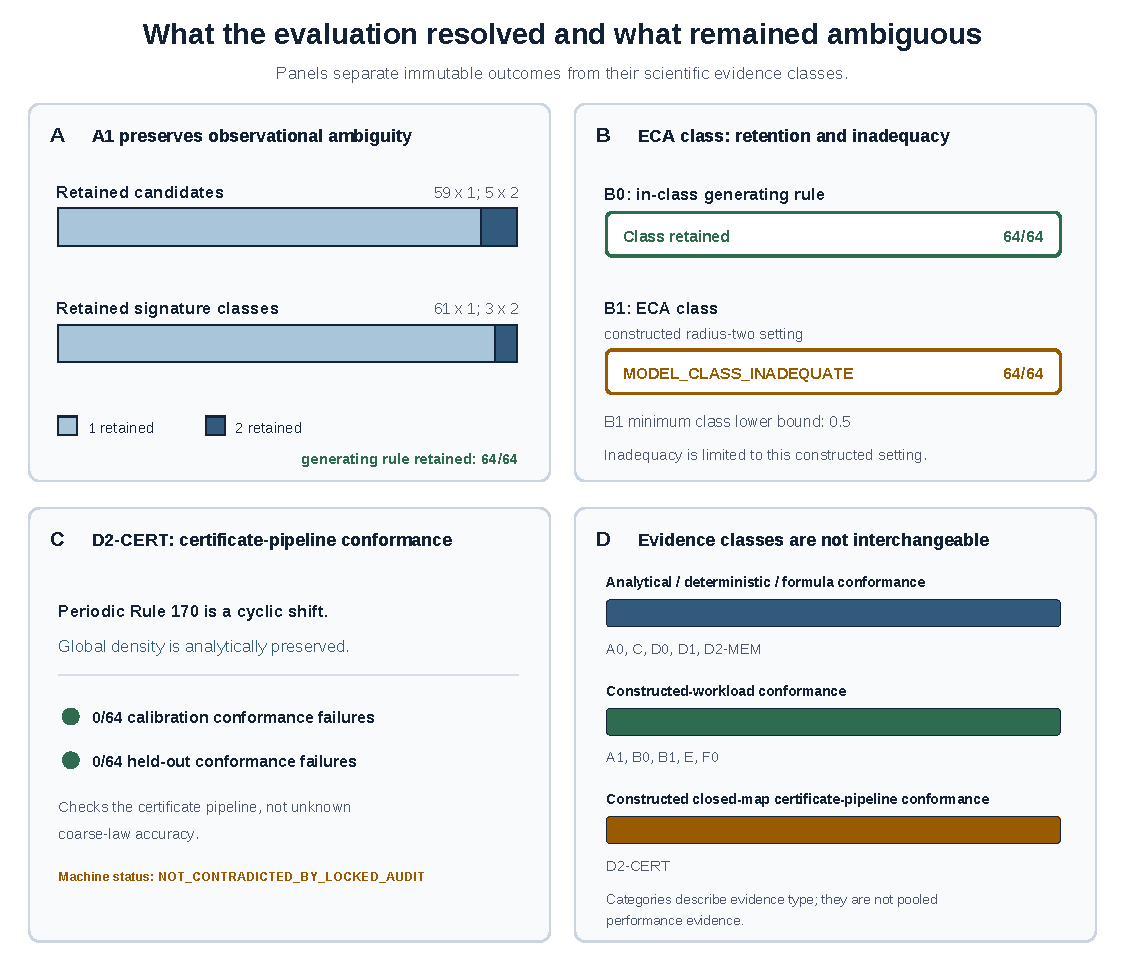
\includegraphics[width=0.96\linewidth]{scientific_result_evidence_classes_v3_7.pdf}
\caption{Scientifically distinct outcomes and evidence classes. A1 preserves set-valued
ambiguity; B0 and B1 contrast in-class retention with one deliberately distinguishable
constructed out-of-class case; D2-CERT exercises certificate grant and withdrawal machinery on
the analytically density-preserving periodic Rule 170 map. The final panel separates
analytical/deterministic checks, constructed-workload conformance, and constructed closed-map
certificate-pipeline conformance; these categories are not pooled into a model-discovery
performance score.}
\label{fig:scientific-results}
\end{figure}

\subsection{Complete accounting exposed ambiguity rather than erasing it}

All 256 ECA rule IDs received a terminal ledger entry. The A0 truth-table and paired
production/reference trajectory census across four specified boundaries---periodic, fixed
zero, fixed one, and edge-replicate (historical code token: \texttt{reflect})---produced 0/256
discrepancies and formed 36 canonical signature classes. The
finite language was fully accounted for under that interface; enumeration beyond the ECA
grammar is outside this claim.
The 36 classes are operational classes induced by the finite probes, quantizers, and serialization
used here. They are neither universal dynamical-equivalence classes of ECA rules nor a standard
symmetry-class count.
Complete accounting supports a statement about coverage of this language; it does not establish
that the language is adequate.

The A1 result was not merely ``the generating rule was found.'' The data-generating rule and its
signature class remained in the retained set in all 64 blocks, with 0 adverse blocks. Yet 59
blocks retained one rule and five retained two; 61 retained one signature class and three
retained two. The finding is set-valued identification under finite observations. It argues for
more discriminating observables when uniqueness matters, rather than a hidden tie-break. The
alternatives are operationally indistinguishable here, not ontologically identical.

For a correct implementation, zero A1 adverse blocks follow from generating each noiseless
history with a member of the enumerated grammar and retaining every candidate with exact loss
zero. The 64-block interval therefore characterizes adverse implementation/accounting events
under the reference role law; it is not an estimate of open-world discovery accuracy. The real
finding remains the set-valued ambiguity that the finite observation interface exposed.

\subsection{The class gate separated a bad model from a bad language}

The paired B endpoints tested opposite constructed cases. In B0, all 64 complete-support in-class blocks
retained the class containing the generating rule. In all 64 complete-support blocks from the
deliberately distinguishable radius-two construction, the ECA class returned \classbad. Every
minimum signature-class lower bound was \(0.5\), above the threshold \(0.2\).
The corresponding B0 minimum was zero, so no in-class block produced false inadequacy.

The gate thus distinguished this constructed out-of-class setting from its in-class control. B1's
outer-XOR generator guarantees disagreement with every radius-one ECA candidate on half of its
complete 32-row support, so the observed 64/64 decision is a conformance check of exact-loss,
complete-ledger, and gate machinery. B1 does not estimate power against arbitrary
misspecification, and the endpoint-wise block interval does not turn it into such an estimate.

\subsection{Error and coarse-graining claims remained conditional on their interfaces}

All nine path-bound cases completed with no violation or domain exit. The
largest raw reference--candidate discrepancy was \(0.1662\), meaningful only in
relation to its stated bound. The smallest margin was near \(-10^{-16}\) and remained within
the fixed \(10^{-12}\) tolerance, so it did not change a decision. These are constructed
implementation checks; full-precision values remain in the Supplement and released source data.
The tolerance governs the comparison at the numerical boundary; it does not turn the nine cases
into a general trajectory-accuracy guarantee.

The deterministic coarse-dynamics checks reproduced Rule 204 full-microstate identity, the Rule
90 density non-closure witness, and exact lag-1 repair in the two-bit memory system. D2-CERT has a
narrower, now explicit evidence class: constructed closed-map certificate-pipeline conformance.
Under periodic boundaries Rule 170 copies the right neighbor, hence performs a cyclic
shift and preserves global binary density exactly. With the registered identity predictor and
zero tolerance, a correctly executed block cannot violate the event. Calibration and held-out
evaluation each observed 0/64 violations, checking role separation, simulator/fidelity agreement,
and the grant/withdrawal pipeline for this construction rather than estimating uncertain
coarse-law accuracy.

The immutable held-out two-sided 95\% interval was \([0,0.0560]\), the one-sided lower endpoint
was zero, and the withdrawal rule did not fire. These exact-binomial values describe a hypothetical
Bernoulli rate of block-level implementation/conformance failure under the iid reference law; they
are not uncertainty about the analytical density identity itself. The exact machine status remains
\texttt{NOT\_CONTRADICTED\_BY\_LOCKED\_AUDIT}. It neither confirms a broader closure theorem nor
grants a new certificate, and it does not transfer to another boundary, coarse variable, or
physical system.

A post-hoc operating-characteristic calculation, using the unchanged \(m_L=64\),
\(\gamma=\delta_{\mathrm{cert}}=0.05\) rule, shows that withdrawal first occurs at \(K_L=7\):
\(L_{\mathrm{CP}}(6,64)=0.04162\) and \(L_{\mathrm{CP}}(7,64)=0.05247\). Its withdrawal probability
is \(0.461\) at a hypothetical implementation-event rate of \(0.10\) and \(0.864\) at \(0.15\).
This calculation is not a registered endpoint and does not change the exact D2 status. Because a
correct implementation cannot violate the registered construction, the grid describes operating
characteristics of the withdrawal machinery under hypothetical faults, not uncertainty about the
Rule 170 density identity.

All prespecified fidelity comparisons preserved their upper-level observables and decisions and
required no further refinement. This conclusion is specific to their observables, tolerances,
horizons, and input laws.
The comparisons distinguish lower-level numerical change from change that matters to the stated
scientific inference.

\subsection{One prespecified order was least costly on this workload}

Both \texttt{fixed\_order} and \texttt{development\_frozen\_order} were distinct permutations of
the same 256 candidates generated before protected execution by sorting salted SHA-256 digests;
neither carried a scientific ordering prior. All four policies matched the exhaustive final
decision, best valid candidate, and failure status in all 64 paired blocks. Their costs nevertheless
differed because the role-derived generating rules occupied different positions in those fixed
permutations: \texttt{fixed\_order} used 75,080
units, development-frozen order 89,816, adaptive fidelity 92,592, and exhaustive search 132,096.
Relative to exhaustive search, the first three saved 43.16\%, 32.01\%, and 29.91\%, respectively.

\begin{figure}[htbp]
\centering
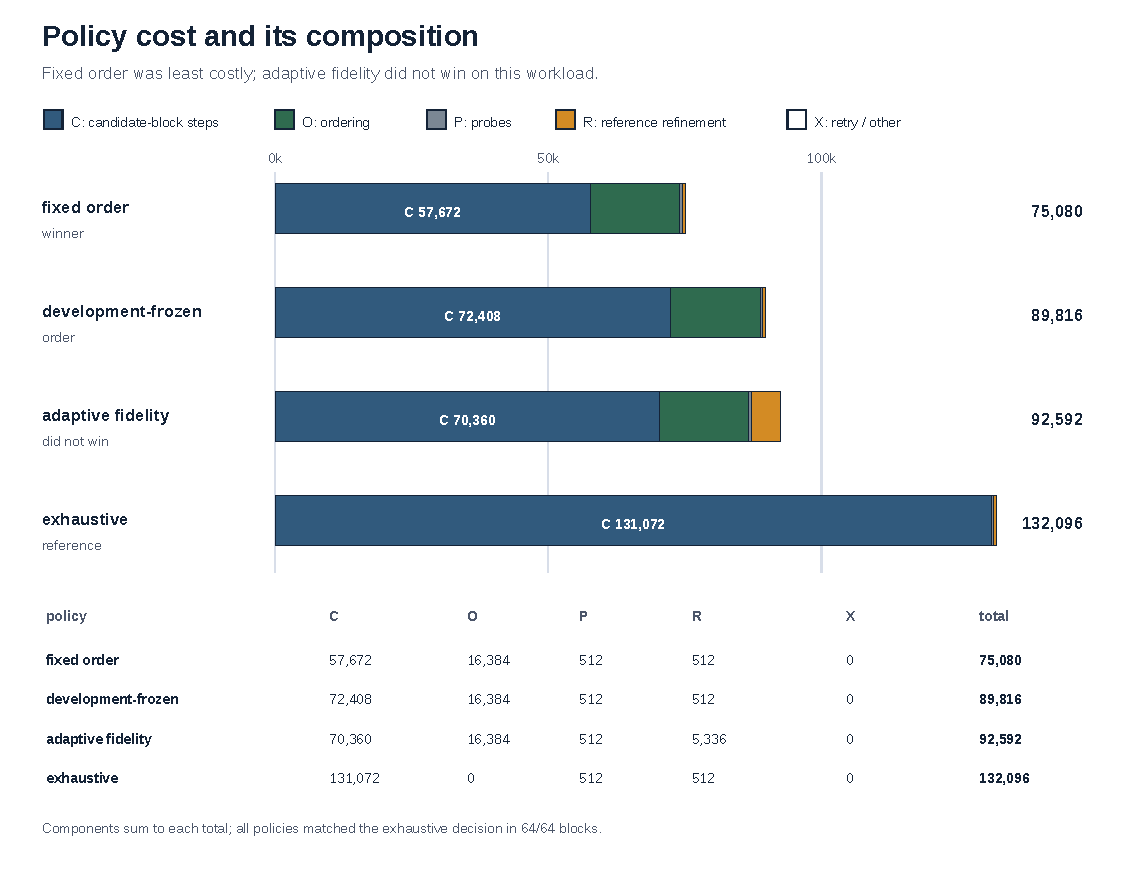
\includegraphics[width=0.95\linewidth]{policy_cost_composition_v3_4.pdf}
\caption{Benchmark E costs on the same 64 observation streams. Stacked components
include candidate-block steps, ordering, probes, reference refinements, and retry/other costs;
they sum to each reported total. All policies agreed with exhaustive search, but one prespecified
salted pseudo-random order was least costly and adaptive fidelity did not win this constructed
workload.}
\label{fig:policy-cost}
\end{figure}

Adaptive fidelity cost about 23.32\% more than \texttt{fixed\_order} and 3.09\% more than
\texttt{development\_frozen\_order}. Its cheap tier evaluates four support rows for all 256
candidates before full-tier evaluation and reference refinement; that overhead was not repaid in
this grammar. The supported conclusion is narrow: one prespecified early-stopping order was least
costly on this constructed workload and registered cost map, while adaptive fidelity did not win.
Cost units are bookkeeping components, not universal wall-clock time, and the ranking does not
generalize to multifidelity search.

\subsection{Known-fixture recovery completed the finite-grammar test, not the biological bridge}

F0 contained 32 clean translations, 16 single-cell perturbations, and 16 negative controls from
project-defined Rule 54/110 whole-trajectory fixtures. The rules are established ECA fixtures
\citep{cook2004,martinez2006}, but the exact seeds and patterns used here were defined by this
project rather than reproduced from literature. Similarity was 1.000 for clean translations,
0.9988 for perturbations, and 0.511--0.554 for negative controls. This passed as known-template
conformance: recognition of project-defined fixtures and controls, not persistent-structure
discovery, prediction, velocity or lifetime estimation, or a novel phenomenon.
The 32/16/16 counts are descriptive realized strata of the prespecified iid mixture, not additional
inferential endpoints, and the comparison concerns whole trajectories only. Because positive
cases are generated from the same registered templates and negative cases from a project-defined
digest construction, the zero adverse blocks are constructed-workload conformance for a correct
matcher, not an estimate of general pattern-discovery performance.

\section{Discussion}

\subsection{Honest outcomes are part of the method}

APHFS preserved outcomes that a success-only pipeline could collapse. A1 retained the generating
rule while admitting residual ambiguity. The constructed B1 class was declared inadequate only
after every member had a valid bound. D2-CERT's constructed closed-map pipeline reached its exact
non-withdrawal state without implying broader confirmation. Each outcome motivates a different
response: collect sharper observations, specify a
broader language in a new study, or retain a conditional statement.

Failure semantics define the same boundary from the other side. An incomplete ledger or invalid
simultaneous bound suspends the class decision; a domain exit withdraws the cross-scale bound.
Rule 90 density non-closure, lag-1 memory repair in the two-bit system, and the distinct Rule 170
certificate interface show why coarse descriptions must be judged by their own maps, domains, and
questions.
This separation turns apparent failure into experimental guidance. Residual ambiguity calls for
more discriminating observables; class inadequacy calls for a newly specified language; and an
indeterminate outcome calls for repairing evidence or computation before making a scientific
claim.

\subsection{Greater complexity is not automatically greater efficiency}

Benchmark E supplies a concrete caution: adaptive fidelity saved resources relative to exhaustive
search, but one salted pseudo-random early-stopping order was cheaper while reaching the same
decisions. The two static orders differed only by prespecified salts, not by a learned scientific
prior. Adaptation helps only when information gains exceed overhead. This constructed comparison
supports neither a universal fixed ordering nor a rejection of multifidelity methods.

\subsection{Conditions under which APHFS would lose practical value}

APHFS would lose practical value if it abstains so often that it cannot guide the next
measurement; if, across registered domain studies, its decisions repeatedly match a much cheaper
baseline without compensating evidential benefit; if reasonable probe changes make the operational
signature partition unstable; if candidate languages repeatedly fail every domain bridge without
producing informative revisions; or if the declared resource burden makes evaluation infeasible.
These are failure criteria for the usefulness of the framework, distinct from failure of one
candidate model. They require future comparative studies rather than reinterpretation of the
current locked blocks.

\subsection{The next registered biochemical bridge}

The next study can be publicly preregistered around a finite enzyme-kinetics grammar that separates
mechanistic mass-action systems from reduced rate laws. Its in-class language would include bounded
Michaelis--Menten, Hill/cooperative, competitive- and noncompetitive-inhibition, substrate-
inhibition, delay, and allosteric candidates, with equations, units, parameter domains, initial
conditions, conservation constraints, and semantic duplicates fixed. A new data-generating law
would define perturbations, substrate and inhibitor levels, sampling times, replicates, batches,
noise, censoring, missingness, and detection limits. Partial steady-state and time-series
concentrations would then test operational non-identifiability, while an explicitly excluded but
distinguishable mechanism could provide a prespecified class-inadequacy challenge.

The study would define a recovery- or homeostasis-relevant upper observable after substrate or
inhibitor perturbation. Solver tolerance, time step, state resolution, and horizon refinements
would be accepted only when that observable and its retain/inadequate/indeterminate decision remain
stable. New development, calibration, and held-out roles would be generated for this study; the
current ECA roles would not be reused. The new protocol would define sample size, power,
multiplicity, stopping, and fair cost accounting before evaluation. AIC, BIC, profile likelihood,
top-1 selection, or SINDy could enter only as prespecified empirical baselines under the same
observations and budgets. Ambiguity, class
inadequacy, fidelity failure, and policy non-advantage would remain admissible rather than being
recoded as success. This blueprint is a future study, not biochemical evidence in the present one.

Repeated bridges of this kind are required before movement toward cellular organization.
Whole-cell models illustrate both integrative reach and demanding validation
\citep{karr2012,thornburg2022,thornburg2026,thornburg2026correction}. Aging becomes testable only
when models predict longitudinal homeostatic drift and recovery under suitable data
\citep{lopezotin2013,lopezotin2023}; rejuvenation follows later through causal,
safety-constrained intervention studies. More classical or quantum compute may expand the
evaluation, but it cannot substitute for domain evidence; no quantum advantage was tested here.

\enlargethispage{2\baselineskip}
\section{Limitations}

The study is deliberately narrow. Completeness applies only to the 256 radius-one binary rule
addresses under the specified interfaces. A0 is internal implementation conformance; C, D0, D1,
and D2-MEM are analytical, deterministic, or formula checks. A1, B0, B1, E, and F0 are constructed
workload-conformance endpoints whose blockwise intervals concern adverse implementation or
accounting events under the reference role law, not general discovery accuracy. B1 is deliberately
distinguishable and F0 uses project-defined fixtures. D2-CERT checks certificate machinery on an
analytically closed Rule 170 density map; its exact status is non-withdrawal, not confirmation.
Endpoint-wise exact-binomial intervals are not a simultaneous family-wide guarantee, and their
exactness applies to the iid reference law with the disclosed conditioning correction for the
implemented roles.

The scalar reference and vectorized production paths were written separately but within the same
project with substantive AI assistance; their agreement is not external replication. Benchmark E's ranking is
specific to two salted pseudo-random orders, one constructed workload, and one cost map. No quantum
interface was implemented, and no external particle, chemical, molecular,
cellular, aging, clinical, or intervention data were analyzed. The present contribution is a
methodological systems-biology architecture and finite ECA machinery test, not a validated domain
model or therapeutic claim.

\section{Data and code availability}

The accompanying Supplement and versioned reproducibility archive provide the executable source
tree, fixed configurations and schemas, environment locks, safe aggregate source tables,
figure-generation code, A0 candidate/signature records, and read-only tools for reconstructing
reported endpoint counts, exact-binomial calculations, aggregate tables, figures, intervals, and
costs. The archive does not rerun the original one-time evaluation and is not an independently
written implementation, new-role replication, or validation on new data. Code is licensed under
the MIT License; the manuscript, documentation, and released aggregate data use CC BY 4.0. A
public repository URL will be added only after the author separately authorizes publication and
verifies the final remote contents.

\section{Declarations}

\paragraph{Intellectual origin and author responsibility.}
Mingyuan Chen conceived the APHFS research program and its central thesis for this project,
selected the scientific questions and claim boundaries, approved the study design, and made the
final scientific judgments. AI systems contributed substantive methodological, formal, software,
and editorial assistance as disclosed below; the author decided what to adopt and accepts
responsibility for the work. This origin statement records authorship of the present APHFS
integration, not historical priority for its established components, automated discovery, or
computational descriptions of nature.

\paragraph{Author contributions.}
Mingyuan Chen: Conceptualization, Methodology, Formal analysis, Validation,
Investigation, Data curation, Visualization, Writing--original draft, Writing--review \& editing,
and Project administration.

\paragraph{Funding.}
No external funding was received for this work.

\paragraph{Competing interests.}
The author declares no competing interests.

\paragraph{Ethics statement.}
Not applicable. This theoretical and computational study used no human participants, human data,
animals, clinical intervention, or identifiable private data.

\paragraph{Acknowledgments.}
None.

\paragraph{AI-assisted technologies.}
The author used OpenAI ChatGPT (primarily GPT-5.6 Sol through the standard and reasoning settings
available in the author's account) and OpenAI Codex for outlining and drafting, methodological and
formal suggestions, software implementation and refactoring, tests, mathematical exposition,
figure preparation, literature organization, adversarial review, release engineering, and
editing. Anthropic Claude (primarily Claude Opus 5 and Claude Fable 5.1) was used for methodological
critique, adversarial review, and revision suggestions. Google Gemini and xAI Grok were used only
for limited exploratory critique; their exact versions were not recorded, and no specific
retained substantive contribution is attributed to them. The model-version history is therefore
partial.

AI outputs were treated as provisional suggestions, not evidence or independent validation.
Mingyuan Chen originated the central research direction, set the scientific questions and claim
boundaries, reviewed the manuscript and reported results, checked the functions and assumptions of
Equations (1)--(10), the Clopper--Pearson calculations, relevant portions of load-bearing sources,
reported file-integrity checks, and directly observed the public read-only aggregate
recomputation. The author has functional-level understanding of the core scientific code but did
not conduct a repository-wide line-by-line review. The author made the final scientific decisions
and accepts responsibility for the work within this disclosed review scope. No human, animal,
clinical, or identifiable private biological data were supplied to these systems. AI systems are
not authors or CRediT contributors.

\section{Conclusion}

APHFS is a discipline for moving from imagination through executable mathematics to evidence.
Bottom-up candidate generation meets top-down reality constraints; complete accounting within a
finite grammar leaves room for ambiguity, whole-class inadequacy, and an indeterminate result.
Coarse-graining is not accepted prematurely, and fidelity is sufficient only when refinements
preserve upper-level observables and decisions. Compute expands evaluation; evidence constrains
justification. A future fault-tolerant quantum layer could expand which pre-particle or
quantum-native dynamics are executable, but it would neither remove the output burden of complete
terminal-ledger accounting nor supply empirical support. Biology, aging, and rejuvenation remain
downstream research destinations.

In the complete 256-rule ECA testbed, the generating rule was retained but was not always unique;
the constructed B1 setting rejected an inadequate class while B0 retained its in-class control;
and the provably density-preserving Rule 170 construction exercised certificate machinery without
withdrawing or confirming a broader claim. All policies agreed with exhaustive search, yet one
prespecified salted pseudo-random order was least costly on this workload and adaptive fidelity did
not win. Ambiguity, constructed scope, and a negative method comparison are part of the result.

The next bridge should test a small biochemical model class with domain observations collected
independently of model development, new role-separated data, protected recovery observables, and
the same permission to fail. Only repeated empirical bridges could justify movement toward
cellular models, aging as loss of resilience, and eventually safety-constrained rejuvenation
research.

\clearpage
\appendix
\section{Supplementary derivations, protocol, and immutable results}
\label{sec:supplement}

This supplement provides derivations, the complete frozen protocol, safe aggregate outcomes, and
provenance commitments for the accompanying APHFS preprint. It reports only safe aggregates and
commitments read from the immutable first-and-only locked result and source data checked by
independent read-only recomputation. The result bundle SHA-256 is
\nolinkurl{6fb3f08e48b4d3496e190fbc38b029ee7c15e327c504924f8c03b6e2083aec9c}, and the
execution-receipt SHA-256 is
\nolinkurl{730bfe099a74b1ccfa281e653e9330bf91a5e73c30b24a58cf52dd88028c4766}.
No raw calibration or locked role value is reproduced here, and no development or public-mock
output is relabeled as scientific evidence. The locked result was not rerun, replaced, tuned, or
used to add a result-dependent endpoint.

\subsection{Finite-class derivation and scheduling}
\label{supp:finite}

For fixed \(h\), Hoeffding's inequality gives \citep{hoeffding1963}
\[
\Pr\!\left(\left|\widehat R_n(h)-R(h)\right|>u\right)
\le 2e^{-2nu^2}.
\]
For the fixed single-valued parser and address set
\(\mathcal A_b=\bigcup_{j=0}^{b}\{0,1\}^j\), the executable semantic image obeys
\[
N_{b,r}=|\mathcal H_{b,r}|\le|\mathcal A_b|=2^{b+1}-1<2^{b+1}.
\]
The ledger itself is address-indexed: invalid and resource-infeasible addresses receive terminal
rows, while parser aliases remain separate unless a canonical-address rule was fixed in advance.
Thus complete accounting is relative to the declared parser/address policy, not to all semantic
models or nature.
Therefore the union bound is
\[
\Pr\!\left(\max_{h\in\mathcal H_{b,r}}
\left|\widehat R_n(h)-R(h)\right|>u\right)
\le 2N_{b,r}e^{-2nu^2}.
\]
Setting
\[
c_b(\delta_{\mathrm{conf}})=
\sqrt{\frac{(b+2)\log2+\log(1/\delta_{\mathrm{conf}})}{2n}}
\]
makes the right-hand side no greater than \(\delta_{\mathrm{conf}}\). The optimizer is required to satisfy
\[
\widehat R_n(\widehat h_n)+\lambda_nL_d(\widehat h_n)
\le \min_{h\in\mathcal H_{b,r}}
\{\widehat R_n(h)+\lambda_nL_d(h)\}+\xi_n.
\]
The three-line comparison in Theorem~\ref{thm:finite} uses \(L_d(h_{b,r}^\star)\le b\),
\(-L_d(\widehat h_n)\le0\), and \(\lambda_n\ge0\). Because
\(\mathcal H_{b,r}\) is explicitly assumed nonempty and finite, its risk minimum is attained;
no infimizing-sequence step is needed. The nonempty registered envelope, common measurable
\([0,1]\)-valued loss interface, and common evaluation distribution are all fixed before and
without using the evaluation sample; that same loss and distribution define every displayed risk. The
inclusion \(\mathcal H_\infty\supseteq\mathcal H_{b,r}\) makes
\(\varepsilon_{\mathrm{app}}(b,r)=R_{b,r}^\star-R_\infty^\star\) nonnegative. The resource vector \(r\)
restricts which descriptions execute, while the displayed cardinality exponent depends only on
the bit budget \(b\).

A sufficient prespecified scheduling regime makes every term on the right side of
Equation~\eqref{eq:oracle} vanish: \(b_n\to\infty\),
\(\varepsilon_{\mathrm{app}}(b_n,r_n)\to0\), \(b_n/n\to0\), \(\delta_{\mathrm{conf},n}\to0\),
\(\log(1/\delta_{\mathrm{conf},n})/n\to0\), and
\(\lambda_nb_n+\xi_n\to0\). This yields convergence in probability relative to the declared
envelope comparator, not natural truth risk or model identification. Almost-sure convergence
additionally needs a summable failure schedule
\(\sum_n\delta_{\mathrm{conf},n}<\infty\). The class, loss, distribution interface, and resource
schedule are fixed before each evaluation sample; the conclusion does not cover adapting a grammar
to the same evaluation data. The schedule need not be nested for the in-probability statement. A separate \(b^{-\nu}\) rate
illustration would additionally require a nested or otherwise monotone approximation structure
that validates the approximation law along the schedule.

\begin{longtable}{>{\bfseries}p{0.19\linewidth}p{0.31\linewidth}p{0.41\linewidth}}
\caption{Notation register for the formal interfaces. Symbols are scoped so that a confidence
level, certificate tolerance, fidelity tolerance, and look index cannot silently exchange
meanings.}\label{tab:notation-register}\\
\toprule
Symbol & Meaning & Scope boundary \\
\midrule
\endfirsthead
\toprule
Symbol & Meaning & Scope boundary \\
\midrule
\endhead
\(a\in\mathcal A_b\) & Declared ledger address & Not the semantic candidate itself.\\
\(r\) & Classical execution-resource envelope & Distinct from the repeated-look radius
\(r_{hgs}\).\\
\(\delta_{\mathrm{conf}}\) & Theorem~\ref{thm:finite} tail-failure probability & Not a
certificate target.\\
\(\varepsilon_{\mathrm{app}}(b,r)\) & Approximation gap to the declared comparison envelope &
Not a certificate or fidelity tolerance.\\
\(\kappa_t\) & Paired-path local discrepancy in Equation~\eqref{eq:path} & Defined at
\(\widehat x_t\) in the registered metric and domain.\\
\(\eta_\ell\) & One-level cross-scale commutation defect & Conditional on typed maps and
admissible intermediate images.\\
\(\varepsilon_{\mathrm{cert}}\) & Coarse-certificate event tolerance & Fixed with the event and
reference law before calibration.\\
\(\delta_{\mathrm{cert}}\) & Certificate grant/withdrawal probability target & Not the theorem
tail probability.\\
\(\varepsilon^{\mathrm{fid}}_j\) & Observable-specific fidelity tolerance & Relative to one
protected observable, horizon, input law, and refinement family.\\
\(s\), \(n_s\) & Registered look index; cumulative observations at that look & Only \(s\)
enters alpha spending; only \(n_s\) enters the radius denominator.\\
\(q_{\mathrm{cal}},q_{\mathrm{locked}}\) & Total-variation bounds induced by role acceptance &
Not quantizers; quantizers retain the notation \(q_j\) only inside Equation~\eqref{eq:signature}.\\
\bottomrule
\end{longtable}

\subsection{Path-error induction}

Let \(e_t=d(x_t,\widehat x_t)\). The triangle inequality, Lipschitz property, and registered
one-step discrepancy yield
\[
\begin{aligned}
e_{t+1}
&=d(F_t(x_t),\widehat F_t(\widehat x_t))\\
&\le d(F_t(x_t),F_t(\widehat x_t))
 +d(F_t(\widehat x_t),\widehat F_t(\widehat x_t))\\
&\le L_te_t+\kappa_t .
\end{aligned}
\]
Repeated substitution gives Equation~\eqref{eq:path}. Here \(\kappa_t\) bounds the second distance
at the candidate-side point \(\widehat x_t\) on the registered paired path in the same metric
\(d\). This deterministic derivation is withdrawn if either trajectory leaves the region on which
\(L_t\) and \(\kappa_t\) are valid or if the local discrepancy was bounded on a different path.

\subsection{Cross-scale composition}

Set
\[
\Gamma_{\ell:\ell}=\mathrm{id}_{X_\ell},\qquad
\Gamma_{\ell:\ell+q}=\Gamma_{\ell+q-1}\circ\cdots\circ\Gamma_\ell\quad(q\ge1).
\]
For every level used below, register the nonempty domain
\[
A_j^{\mathrm{comm}}=\{z\in A_j\cap B_j:
F_j(z)\in B_j,\ \Gamma_j(z)\in A_{j+1}\},
\]
so both compositions in the definition of \(\eta_j\) are typed. For the particular
\(x\in A_\ell^{\mathrm{comm}}\), assume for every \(q=0,\ldots,r-1\) that
\(\Gamma_{\ell:\ell+q}(x)\in A_{\ell+q}^{\mathrm{comm}}\), and assume both
\(\Gamma_{\ell:\ell+q}F_\ell(x)\) and
\(F_{\ell+q}\Gamma_{\ell:\ell+q}(x)\) lie in the registered region on which
\(\Gamma_{\ell+q}\) has constant \(G_{\ell+q}\).
For \(r=1\), Equation~\eqref{eq:cross} is exactly the definition of \(\eta_\ell\).
Assume the result for \(r\). Insert
\(\Gamma_{\ell+r}F_{\ell+r}\Gamma_{\ell:\ell+r}(x)\) between the two terms at
level \(\ell+r+1\). The Lipschitz property of \(\Gamma_{\ell+r}\) multiplies the existing
\(r\)-level discrepancy by \(G_{\ell+r}\), while the newly inserted one-step commutation
term is at most \(\eta_{\ell+r}\). Hence
\[
E_{r+1}\le G_{\ell+r}E_r+\eta_{\ell+r},
\]
which expands to Equation~\eqref{eq:cross} for \(r+1\). This induction proves the displayed
weighted sum. The empty product preserves the newest defect with coefficient one. There is no
initial mismatch because both sides begin at the same \(x\); different starting states invoke the
separate path bound. Every composition must type-check, and every quantified intermediate image
and paired point must satisfy its registered admissibility/Lipschitz premise. If even one premise
is false or unrecorded, the only valid output is
\texttt{CROSS\_SCALE\_BOUND\_WITHDRAWN}; no finite bound may be returned.

\subsection{Exact-binomial coverage and the zero-violation threshold}

For fixed \(C,F_C,D,\varepsilon_{\mathrm{cert}},Q\), let \(W_i\overset{\mathrm{iid}}{\sim}Q\) under the
reference law and define
\[
V_i=\mathbf 1\{D(W_i)>\varepsilon_{\mathrm{cert}}\}
\]
so that the indicators \(V_i\) are iid Bernoulli with parameter
\(p_Q=\Pr_Q\{D(W)>\varepsilon_{\mathrm{cert}}\}\). The one-sided Clopper--Pearson construction in
Equation~\eqref{eq:cp} inverts an exact binomial test and has coverage at least \(1-\beta\)
\citep{clopper1934}.
Consequently, the decision \(U_{\mathrm{CP}}\le\delta_{\mathrm{cert}}\) supports
\(p_Q\le\delta_{\mathrm{cert}}\) at that confidence level. At \(K=0\), solving
\(1-\beta^{1/m}\le\delta_{\mathrm{cert}}\) gives
\[
m\ge \left\lceil\frac{\log\beta}{\log(1-\delta_{\mathrm{cert}})}\right\rceil.
\]
Substitution of \(\beta=\delta_{\mathrm{cert}}=0.05\) yields \(m\ge59\). This threshold is the minimum block count
for the \(K=0\) design case; a design that permits \(K>0\) requires a separate calculation. It is
a planning result under the iid reference law rather than an empirical estimate or an outcome-
dependent stopping rule: the upper endpoint is \(0.05033933833042015\) at \(m=58\) and
\(0.049507609888227\) at \(m=59\). The actual calibration and held-out counts were each fixed at
64; neither stopped after observing 59 zeroes. In the
subsequently authorized first-and-only
locked audit, A1, B0, B1, E, and F0 each observed zero adverse blocks among 64, giving the
endpoint-wise one-sided 95\% upper endpoint
\(0.04572970233076246\) and descriptive two-sided 95\% interval
\([0,0.05600908938663657]\). D2-CERT separately observed zero violations among 64, giving the
endpoint-wise two-sided 95\% interval \([0,0.05600908938663657]\), a one-sided locked lower
endpoint of zero, and no withdrawal. These intervals are not a family-wide 95\% APHFS guarantee.
For A1, B0, B1, E, and F0, the block event is a frozen constructed-workload
implementation, accounting, fidelity, or decision-conformance event; the interval does not convert
any of those endpoints into an estimate of open-world discovery, model-class power, search-policy
superiority, or biological performance.

For D2-CERT, however, the registered scientific event is constructive. With the project's Wolfram
bit convention, Rule 170 returns the right-neighbor bit. Periodic boundaries therefore give
\((F_{170}x)_j=x_{j+1\bmod w}\), a cyclic permutation, so global density is exactly invariant for
every binary initial state and time. The coarse predictor is identity and the event tolerance is
zero. A violation is impossible for a correct implementation; the 0/64 calibration and 0/64
held-out records exercise certificate-state, role-separation, and paired simulator/fidelity
machinery under this proved closure. Their CP calculations may describe a hypothetical block-level
implementation/conformance-failure rate under the iid reference law, but not uncertainty about the
density identity. This evidence class is
\emph{constructed closed-map certificate-pipeline conformance}; the immutable machine
status remains \texttt{NOT\_CONTRADICTED\_BY\_LOCKED\_AUDIT}.

The actual successful role manifests follow this iid reference law conditioned on materializer
acceptance. Calibration required 64 distinct 256-bit values; a union bound gives
\[
q_{\mathrm{cal}}\le {64\choose2}2^{-256}=2016/2^{256}
=1.74105158070704\times10^{-74}.
\]
The held-out role additionally had to avoid all 64 calibration values, giving
\[
q_{\mathrm{locked}}\le\left[{64\choose2}+64^2\right]2^{-256}
=6112/2^{256}=5.27842622087372\times10^{-74}.
\]
Conditioning means the implemented laws are not literally iid. By total variation, the reference-
law coverage guarantees transfer conservatively as at least
\(1-\beta-q_{\mathrm{cal}}\) and \(1-\gamma-q_{\mathrm{locked}}\). The tiny corrections alter no
reported interval, threshold, decision, or status.

Calibration grants only the statement defined by Equation~\eqref{eq:cp}: for the frozen violation
event under the iid reference law \(Q\), the one-sided upper endpoint covers \(p_Q\), and the certificate is
granted only when that endpoint is at most \(\delta_{\mathrm{cert}}\). The separately authorized locked audit
evaluated a different question: whether a held-out, role-separated violation count contradicted
\(p_Q\le\delta_{\mathrm{cert}}\) under its frozen decision rule. It reports a two-sided exact interval and the
one-sided lower endpoint in
Equation~\eqref{eq:cp-audit}. The certificate is withdrawn only when that lower endpoint exceeds
\(\delta_{\mathrm{cert}}\); a raw locked fraction above \(\delta_{\mathrm{cert}}\) is not itself mathematical disproof. Failure to
reject is labeled not contradicted, not confirmed.

Public-mock calibration reports only
\texttt{PUBLIC\_MOCK\_CALIBRATION\_CRITERION\_MET} or its not-met counterpart and never grants a
certificate. An actual grant is new-written as an immutable certificate record binding the
approved freeze, runtime inventory, protocol/config/fidelity hashes, calibration role commitment,
complete result bundle, separate \(\beta\) and \(\gamma\), exact event, \(Q\), and no-retuning
declaration; the completed workflow created that record and completed its documented calibration-review
step before locked authorization. Locked D2 is inapplicable without that granted record plus a
schema-valid calibration-review approval bound to the raw result and certificate; it cannot grant a certificate. The four
state fields \texttt{calibration\_executed}, \texttt{locked\_audit\_executed},
\texttt{certificate\_granted}, and \texttt{certificate\_reviewed} are separate facts and may not
be inferred from one another.

\paragraph{Post-hoc D2 withdrawal-rule operating characteristics.}
This paragraph and Table~\ref{tab:d2-power} carry the labels
\nolinkurl{POST_HOC_OPERATING_CHARACTERISTIC_ANALYSIS},
\nolinkurl{NOT_A_PREREGISTERED_ENDPOINT}, and
\nolinkurl{DOES_NOT_CHANGE_D2_STATUS}. For \(m_L=64\),
\(\gamma=\delta_{\mathrm{cert}}=0.05\), the frozen one-sided lower-bound rule first satisfies
\(L_{\mathrm{CP}}(K_L,64;0.95)>0.05\) at \(K_L=7\):
\[
\begin{aligned}
L_{\mathrm{CP}}(6,64;0.95)&=0.04161966005858663,\\
L_{\mathrm{CP}}(7,64;0.95)&=0.05247175276586141.
\end{aligned}
\]
Thus the trigger event is \(K_L\ge7\). Under a hypothetical true violation probability \(p\),
its withdrawal probability is the binomial tail
\[
\Pr_p(K_L\ge7)=1-\sum_{j=0}^{6}{64\choose j}p^j(1-p)^{64-j}.
\]
The domain is a hypothetical iid Bernoulli sequence of block-level implementation/event-mechanism
failures governed by the unchanged rule. The calculation does not reuse role values, is not
evidence about the observed blocks, and is not uncertainty about Rule 170's analytical identity.

\begin{table}[htbp]
\centering
\caption{Post-hoc operating characteristics of the unchanged D2-CERT withdrawal machinery under
hypothetical block-level failures. Values are deterministic binomial-tail calculations, not new
endpoint outcomes or evidence against the proved Rule 170 density identity.}\label{tab:d2-power}
\begin{tabular}{ccc}
\toprule
Hypothetical block-failure rate \(p\) & Trigger & Withdrawal probability \\
\midrule
0.05 & \(K_L\ge7\) & 0.0402969 \\
0.08 & \(K_L\ge7\) & 0.2498734 \\
0.10 & \(K_L\ge7\) & 0.4609612 \\
0.12 & \(K_L\ge7\) & 0.6602532 \\
0.15 & \(K_L\ge7\) & 0.8635388 \\
0.20 & \(K_L\ge7\) & 0.9817801 \\
\bottomrule
\end{tabular}
\end{table}

\begin{table}[htbp]
\centering
\caption{\(K=0\) sample-size planning at \(\beta=0.05\). Each entry is the smallest integer
\(m\) satisfying \(1-\beta^{1/m}\le\delta_{\mathrm{cert}}\); designs allowing violations require a different
calculation.}\label{tab:k0-planning}
\begin{tabular}{cc}
\toprule
Target \(\delta_{\mathrm{cert}}\) & Minimum \(m\) for the \(K=0\) design \\
\midrule
0.05 & 59 \\
0.02 & 149 \\
0.01 & 299 \\
0.005 & 598 \\
0.001 & 2995 \\
\bottomrule
\end{tabular}
\end{table}

\paragraph{Post-hoc multiplicity sensitivity.}
The registered endpoint-wise summaries remain controlling. As an illustrative
\texttt{POST\_HOC\_MULTIPLICITY\_SENSITIVITY}, allocating a total one-sided tail probability
0.05 equally across the five homogeneous \(K=0,m=64\) zero-adverse blockwise conformance
endpoints under the iid reference law gives
\(\beta^\star=0.01\) and
\[
1-(0.01)^{1/64}=0.06942795907030102.
\]
This Bonferroni calculation requires each component interval's own binomial assumptions but not
independence among endpoints. It was not registered, changes no status, and is not substituted for
the endpoint-wise \(0.04572970233076246\). A calculation treating all eleven endpoints as
homogeneous is not reported as a family-wide result because five are deterministic or
formula-conformance checks, D2-CERT uses a different direction and role, and the endpoints do not
share one estimand.

\subsection{Proposed APHFS-Q execution contract}
\label{supp:quantum-contract}

This subsection is \texttt{PROPOSED\_QUANTUM\_EXTENSION} and \texttt{ROADMAP\_ONLY}. It defines an
interface for a future separately registered study; it reports no quantum execution, resource
estimate, endpoint, or scientific result. The scientific logic---declared candidate language,
complete accounting or disclosed sampling, operational ambiguity, class inadequacy,
indeterminacy, fidelity withdrawal, and role-separated evaluation---is hardware-independent.

\begin{longtable}{>{\bfseries}p{0.20\linewidth}p{0.47\linewidth}p{0.25\linewidth}}
\caption{Typed \(\mathsf{QuantumResourceRecord}\) for a future execution contract.}\label{tab:q-contract-full}\\
\toprule
Field & Registered content & Missing/failed action \\
\midrule
\endfirsthead
\toprule
Field & Registered content & Missing/failed action \\
\midrule
\endhead
\texttt{semantics} & Finite or sampled grammar, canonical encoding, valid-state rules, and
unitary, CPTP channel, Hamiltonian, circuit, quantum-walk, or QCA update semantics. & Reject invalid
candidates; do not impute a favorable status.\\
\shortstack[l]{\texttt{input\_and}\\\texttt{\_preparation}} & Input origin, normalization, preparation circuit/channel,
construction cost, target error, success probability, repetitions, and reusability. &
\texttt{INDETERMINATE} if correctness or cost is unsupported.\\
\texttt{operator\_access} & Oracle, sparse access, LCU, block encoding, product formula, or other
access model, including normalization, construction/query cost, error, and reuse assumptions. &
Mark access-infeasible or \texttt{INDETERMINATE}.\\
\texttt{logical\_circuit} & Logical qubits, fixed native logical gate basis, gate counts/depth,
circuit family, synthesis tolerance, and termination budget. Toffoli is either native or compiled
to T gates, never charged twice. & Mark resource-infeasible or reject an untyped record.\\
\texttt{qec\_mapping} & Code family, distance, physical-noise model, decoder, factories,
layout/connectivity, cycle time, and logical-failure allocation. & \texttt{INDETERMINATE} without
an instance-specific mapping.\\
\texttt{physical\_estimate} & Derived physical-qubit, cycle, wall-time, energy where available,
and factory estimates, reported as ranges or confidence statements. & Do not present a point
estimate as exact or mix it with logical counts.\\
\shortstack[l]{\texttt{measurement}\\\texttt{\_and\_readout}} & Observables, shots, estimators, simultaneous intervals,
quantization grid, guard bands, device readout, and mitigation. & Return
\texttt{SIGNATURE\_INDETERMINATE} when an interval touches a cell boundary.\\
\shortstack[l]{\texttt{classical}\\\texttt{\_postprocessing}} & Decoding, estimator evaluation, result verification,
terminal-record materialization, storage, communication, and classical wall time. & Mark
incomplete cost or output; do not hide classical work.\\
\texttt{error\_budget} & Preparation, access, simulation, synthesis, logical/QEC, sampling,
readout, classical-processing, and coarse-graining errors, each with domain and metric. & Withdraw
the affected inference or return \texttt{INDETERMINATE}.\\
\texttt{provenance} & Candidate/config/software/hardware/calibration identifiers, compiler and
mapping versions, hashes, failure records, and classical comparator. & No advantage,
reproducibility, or domain claim without a complete binding.\\
\bottomrule
\end{longtable}

Guard-banded signatures retain exact partition semantics only after statistical determination:
each simultaneous interval must lie wholly inside one prespecified quantization cell; otherwise
the candidate remains signature-indeterminate. This construction is a proposal, not a proved or
tested theorem. Likewise, no generic formula such as independent, equal logical-gate failure is
assumed. Probability terms may be combined by a valid proved bound or union bound only when their
events and assumptions are registered; quantities in different metrics remain separate.

These typed records are compared componentwise, with Pareto dominance as the default. A scalar
total is permitted only when its cost map, units, exchange rates, uncertainty treatment, and
classical baseline were prespecified. Physical-qubit requirements are derived from
\texttt{qec\_mapping}, not stored as a union-type alternative to a QEC model. The native logical
gate basis determines whether Toffoli is primitive or decomposed into T gates, preventing double
counting. Preparation, access, measurement/readout, terminal-record output, verification, storage,
and classical wall time are part of the end-to-end resource statement rather than free peripherals.

\begin{table}[htbp]
\centering
\small
\caption{Falsifiable milestones for a future quantum execution program.}\label{tab:q-milestones}
\begin{tabularx}{\linewidth}{>{\bfseries}p{0.08\linewidth}p{0.25\linewidth}p{0.37\linewidth}p{0.20\linewidth}}
\toprule
Stage & Candidate object & Required evidence & Failure action \\
\midrule
Q0 & Small local unitary or QCA & Exact classical small-instance encoding cross-check &
Reject encoding \\
Q1 & Fixed quantum candidate & Instance-specific logical qubits, depth, non-Clifford count,
shots, and QEC model & Mark resource-infeasible \\
Q2 & Registered observable & Classical/quantum comparison for the same observable and tolerance &
Withdraw fidelity \\
Q3 & Finite quantum-native grammar & New-role ambiguity and whole-class gate &
Retain set, reject class, or abstain \\
Q4 & Physical or chemical signature & Independently collected domain observations &
Reject or revise the candidate class \\
Q5 & Reaction or molecular class & Separate publicly preregistered future biological study &
No biological claim from earlier stages \\
\bottomrule
\end{tabularx}
\end{table}

Candidate classes must also state which physical premises they adopt: locality/causality,
no-signalling, symmetry/isotropy, unitarity or CPTP dynamics, conservation, continuum-limit
dispersion, and the relevant scattering or spectroscopic constraints. Bell's theorem constrains
local hidden-variable accounts under its assumptions \citep{bell1964}; it does not force all
pre-particle grammars to be QCA. QCA remains one candidate family with substantial direct prior
art \citep{watrous1995qca,meyer1996qca,bialynicki1994,schumacher2004,
arrighi2011localizability,gross2012qcaindex,darianoperinotti2014,
darianoperinotti2017,farrelly2020}.

\begin{longtable}{>{\bfseries}p{0.19\linewidth}p{0.29\linewidth}p{0.43\linewidth}}
\caption{Concrete direct-method comparison. This replaces broad capability checkmarks with the
premise and conclusion of a cited procedure; no row assigns APHFS an intrinsic advantage.}
\label{tab:direct-method-comparison}\\
\toprule
Procedure & Direct precedent and premise & Relation to the proposed APHFS integration \\
\midrule
\endfirsthead
\toprule
Procedure & Direct precedent and premise & Relation to the proposed APHFS integration \\
\midrule
\endhead
Cellular-automaton coarse-graining & Israeli and Goldenfeld construct coarse descriptions and
study predictability for cellular automata \citep{israeli2004,israeli2006}. & Directly precedes
coarse-graining of ECA. APHFS adds a proposed requirement to bind acceptance to stated domains,
upper observables, tolerances, and decisions; the present ECA checks are not biological
multiscale validation.\\
Version spaces and candidate elimination & Candidate elimination maintains the hypotheses
consistent with examples, and generalization is framed as search in a hypothesis space
\citep{mitchell1977candidate,mitchell1982}. & Directly precedes retained candidate sets. APHFS's
additional proposal is address-level terminal accounting and explicit failure/class-inadequacy
semantics, not priority for set-valued search.\\
Finite-program synthesis & Sketching and syntax-guided synthesis search grammar-constrained
programs; unrealizability logic can prove that no program in a grammar satisfies a specification
\citep{solarlezama2006,alur2013sygus,kim2023unrealizability}. & These are formal-specification
procedures. APHFS instead proposes separating an executable grammar from empirical evidence and
statistical class bounds; synthesis realizability is not empirical adequacy.\\
Partial identification and model confidence sets & Partial identification and model-confidence-
set procedures return sets under their own sampling and decision assumptions
\citep{manski2003,hansen2011mcs}. & They directly precede set-valued conclusions. APHFS operational
signatures, retained candidates, and class-inadequacy gate have different estimands and must not be
presented as replacements for those methods.\\
Goal-oriented error control & Quantity-of-interest error estimation, including a lattice-model
extension, protects selected outputs rather than every microscopic value
\citep{prudhomme1999goal,oden2005lattice}. & This directly precedes observable-relative numerical
control. APHFS proposes linking it to candidate decisions and failure records; it does not claim
the underlying principle as new.\\
Systems-biology identifiability & Structural and practical identifiability analyze whether
parameters or combinations are determined under a specified model and observation design
\citep{bellman1970identifiability,chis2011,gutenkunst2007,raue2009,villaverde2016}. & APHFS's
finite whole-candidate signature is a neighboring operational object, not a substitute for
parameter identifiability and not biological validation.\\
QCA and discrete quantum dynamics & One-dimensional QCA, quantum lattice gases, localizability,
and index theory formalize specific local quantum dynamics
\citep{watrous1995qca,meyer1996qca,arrighi2011localizability,gross2012qcaindex}. & These are direct
predecessors of any future quantum candidate grammar. APHFS claims only a proposed accounting,
failure, fidelity, and evidence interface around such candidates.\\
End-to-end fault-tolerant resources & State preparation, surface-code mapping, and instance-level
resource studies expose costs omitted by query counts
\citep{pleschbrukner2011,fowler2012surface,gidneyekera2021,lowchuang2019,reiher2017,
liu2024,eklund2026}. & They motivate
the typed resource record. No APHFS quantum implementation, instance estimate, or advantage was
performed here.\\
\bottomrule
\end{longtable}

\subsection{Frozen split roles}
\label{supp:splits}

The completed protected workflow retained the frozen role separation. D2-CERT alone used 64
calibration blocks. A1, B0, B1, D2-CERT, E, and F0 each used 64 locked blocks; A0, C, D0, D1,
and D2-MEM used their registered deterministic or complete finite censuses. The calibration role
was materialized once and calibration was executed once in the earlier authorized phase. The
locked role was materialized once and the locked audit was executed once. Neither role was
rematerialized, replaced, or reordered; neither protected execution was retried. Raw role values
remained sealed through confirmatory execution, separate result review, and independent read-only
recomputation of safe artifacts. They were approved
for subsequent release only as \texttt{POST\_AUDIT\_REPRODUCTION\_ONLY}; any replay is
non-confirmatory and cannot replace the immutable result. No such replay was run for this release
candidate.

Role materialization enforced within-role uniqueness and calibration--locked nonintersection.
Consequently, the implemented role laws are the ideal iid reference laws conditioned on no
collision. The union-bound
total-variation deviations are at most
\(q_{\mathrm{cal}}\le1.74105158070704\times10^{-74}\) and
\(q_{\mathrm{locked}}\le5.27842622087372\times10^{-74}\). These disclosed conditioning terms do
not change any numerator, denominator, Clopper--Pearson interval, threshold, or decision.

\begin{longtable}{>{\bfseries}p{0.14\linewidth}p{0.32\linewidth}p{0.45\linewidth}}
\caption{Completed data-role separation and prohibited reuse.}\label{tab:splits}\\
\toprule
Role & Permitted use & Prohibited use\\
\midrule
\endfirsthead
\toprule
Role & Permitted use & Prohibited use\\
\midrule
\endhead
Development & Choose grammar features, probes, quantizers, maps, thresholds, and proposed filter order. &
Claim locked performance or calibrate the final Clopper--Pearson certificate.\\
Calibration & For D2-CERT only, evaluate the already frozen violation event under registered \(Q\); compute
\(U_{\mathrm{CP}}\). &
Modify \(C,F_C,D,\varepsilon_{\mathrm{cert}},Q\), probes, memory lag, or the certificate threshold.\\
Locked audit & Evaluate the complete frozen decision pipeline once under the signed manifest;
report the exact interval and frozen withdrawal decision. &
Select candidates, tune thresholds, repair failures, or rerun until favorable.\\
Exploratory follow-up & Diagnose a failure and propose a new version. &
Replace the original locked result or inherit its confirmatory label.\\
\bottomrule
\end{longtable}

\subsection{Complete frozen endpoint and fidelity protocol}
\label{supp:protocol}

Table~\ref{tab:full-protocol} preserves the implementation-facing details moved out of the main
scientific narrative. Nothing in this registry was changed after the locked outcome.

For A0, \emph{production/reference} denotes implementation-path separation, not independent
origin. The scalar reference uses an explicit \(111\)-to-\(000\) rule-string lookup and a per-cell
update; the NumPy-vectorized production path uses bit indexing. They do not share rule-lookup or
one-step update functions, but both were developed within the same project under the same
specification with substantive AI assistance. The comparison is therefore an internal
deterministic implementation-conformance check, not an externally authored implementation or
independent replication. Legacy frozen field names containing \emph{independent} are retained as
immutable schema labels and are interpreted only in this narrower sense.
The frozen boundary token \texttt{reflect} implements edge replication: an out-of-range neighbor is
set to the nearest boundary cell, not to the next interior cell of a mirror-reflected array. The
scientific description therefore uses \emph{edge-replicate} while retaining the historical token
where exact code/configuration identity matters.

\begingroup
\scriptsize
\setlength{\tabcolsep}{3pt}
\begin{longtable}{>{\bfseries}p{0.07\linewidth}p{0.20\linewidth}p{0.22\linewidth}
p{0.23\linewidth}p{0.19\linewidth}}
\caption{Complete frozen benchmark protocol and failure interpretation.}\label{tab:full-protocol}\\
\toprule
ID & Registered target & Observation unit and sample & Decision rule & Failure interpretation\\
\midrule
\endfirsthead
\toprule
ID & Registered target & Observation unit and sample & Decision rule & Failure interpretation\\
\midrule
\endhead
A0/A1 & Complete 256-rule ECA accounting; data-generating-rule and signature-class retention &
A0 is a deterministic 256-rule truth-table and paired production/reference trajectory census over
periodic, fixed-zero, fixed-one, and edge-replicate boundaries (historical code token:
\texttt{reflect}). A1 uses 64 locked role-derived blocks under its separately registered
boundary/trajectory interface and no calibration blocks. Blocks, not cells or times, are the
observation units. Its reference block law is iid; the implemented law is that law conditioned on
role uniqueness and calibration nonoverlap. &
Exact candidate losses and a constructed-retention conformance event; endpoint-wise one-sided 95\%
CP upper bound under the iid reference law. &
Missing candidate/class, generating-class omission, failed execution, fidelity instability, or
incomplete ledger is adverse. Multiplicity is retained rather than forced to one.\\
B0/B1 & Avoid false class inadequacy in-class and detect the constructed
\(y=o_L\oplus o_R\oplus f_\theta(l,c,r)\) family &
Each role value creates one distinct complete-support block; 64 locked blocks and no calibration
blocks per endpoint. These are constructed workloads under the same reference/conditioned role-law
distinction. &
Exact complete-support candidate losses and singleton-class minima; B1 threshold \(0.2\);
endpoint-wise CP conformance summary across blocks. &
Missing coverage or an invalid bound is indeterminate. False B0 rejection or a retained/
indeterminate B1 decision is adverse.\\
C & Path-bound conformance for contractive, neutral, and expanding maps under three perturbation
types &
Nine deterministic constructed cases and 81 comparison points; no calibration or locked
randomness. &
Deterministic inequality with frozen \(10^{-12}\) comparison tolerance; domain exit is never
clipped. &
Any bound violation or unregistered domain exit is adverse.\\
D0--D2 & Rule 204 identity, Rule 90 density non-closure, Rule 170 global-density certificate
machinery, and two-bit memory repair &
D0, D1, and D2-MEM are deterministic. D2-CERT alone uses 64 calibration and 64 locked blocks under
the reference/conditioned role-law distinction. &
D2-CERT uses Equations~\eqref{eq:cp} and \eqref{eq:cp-audit}; D2-MEM requires lag-0 ambiguity and
exact lag-1 repair. &
D2-CERT is constructed closed-map certificate-pipeline conformance under the provably closed periodic Rule 170 density
map; its exact status is a distribution-conditional non-withdrawal state, not confirmation. Missing
support, fidelity instability, or incomplete records cannot pass.\\
E & Compare exhaustive, fixed-order, development-frozen-order, and adaptive-fidelity policies &
The same truth-table observation stream and 64 locked blocks; no calibration blocks. Both static
orders are distinct salted-SHA-256 pseudo-random permutations fixed before protected execution;
neither encodes a scientific ordering prior. &
Every candidate-block step, ordering action, probe, reference refinement, retry, and termination
cost is billed under the registered bookkeeping map. Policy agreement is constructed-workload
decision conformance; totals and policy ranking are descriptive and not wall-clock estimates. &
Decision disagreement, unbilled access in the recorded trace, budget breach, missing trace, or unstable fidelity is
adverse.\\
F0 & Recover project-defined Rule 54/110 whole-trajectory fixtures &
Each of 64 locked blocks draws one project-defined fixture case from the iid reference mixture;
the implemented law is conditioned on role acceptance. Realized counts were 32 clean translations,
16 perturbations, and 16 negative controls. &
Endpoint-wise constructed-fixture conformance-failure summary under the iid reference law; realized
strata are descriptive. &
No velocity, lifetime, held-out prediction, persistent detection, literature-seed provenance, or
novel-discovery claim is registered.\\
\bottomrule
\end{longtable}
\endgroup

\begin{table}[htbp]
\centering
\scriptsize
\caption{Benchmark-specific fidelity profiles. Sufficiency is assessed at protected
upper-level observables and decisions, not by raw datatype proximity.}
\label{tab:full-fidelity}
\begin{tabularx}{\linewidth}{>{\bfseries}p{0.16\linewidth}
>{\raggedright\arraybackslash}p{0.23\linewidth}
>{\raggedright\arraybackslash}p{0.25\linewidth}X}
\toprule
Profile & Registered/reference tiers & Protected observable & Failure action\\
\midrule
A1 / D0--D2 & Same-block vector/scalar ECA evaluators; fixed Rule 204/90/170 identities &
Candidate/class retention, complete microstate, density event, or memory-lag decision &
Preserve paired records; instability is adverse; missing refinement is indeterminate.\\
B0 / B1 / C & Bit-index vs explicit-string; vector vs scalar; decimal-6 float vs decimal-12
\texttt{Decimal} &
Exact candidate losses, class decision, bound violation, and domain exit &
Missing support or tier disagreement is indeterminate; domain exit withdraws; never clip.\\
E / F0 & Lazy cheap/full/reference evaluation; vector/scalar template conformance &
Policy decision, best candidate, complete cost ledger, and fixture/control decision &
Hidden cost, tier disagreement, or changed decision is adverse.\\
\bottomrule
\end{tabularx}
\end{table}

\subsection{Candidate, gate, and look ledger}

The registered machine-readable candidate and look ledgers contain at least:
\[
\begin{split}
(&\texttt{run\_id},\texttt{config\_hash},\texttt{source\_hash},
\texttt{candidate\_id},\texttt{description\_bits},\texttt{rule\_id},\\
&\texttt{parse\_status},\texttt{execution\_status},\texttt{signature\_id},
\texttt{representative\_id},\texttt{resource\_usage},\texttt{gate\_id},\\
&\texttt{look},\texttt{sample\_count},\texttt{split\_id},
\texttt{alpha\_allocated},\texttt{bound\_lower},\texttt{bound\_upper},\\
&\texttt{threshold},\texttt{decision},\texttt{seed\_block},
\texttt{precision\_id},\texttt{failure\_code},\texttt{timestamp}).
\end{split}
\]
This tuple is the general framework interface, not a claim that every field drove the immutable
study. The repeated-look construction in Equation~\eqref{eq:alpha} was not in the protected
execution call graph. In that equation the radius denominator is the cumulative sample size
\(n_s\) available at look \(s\), not the look index \(s\) itself. Protected B0/B1 instead used
exact complete-support candidate losses, and every registered signature class in those gates was a
singleton. The frozen \texttt{alpha\_ledger\_complete} field records complete 256-candidate
coverage; it does not establish that the repeated-look allocation was exercised. Consequently,
the class minima in Equation~\eqref{eq:inadequacy} equal their candidate losses here. Neither its
non-singleton aggregation case nor Equation~\eqref{eq:alpha}'s repeated-look radius generated an
immutable endpoint result.
The release-source correction is recorded as
\texttt{POST\_RESULT\_FORMAL\_CORRECTION} and
\texttt{NO\_LOCKED\_ENDPOINT\_DEPENDED\_ON\_THIS\_DISPLAY}; the historical frozen source remains
unchanged.

In an exhaustive run, each addressable description has exactly one terminal
\texttt{execution\_status} under the accounting rule in Section~\ref{sec:six-steps}. The ECA
registry has exactly 256
rule IDs. \texttt{CANONICAL\_DUPLICATE} requires a representative pointer and proof of equality on
the full registered evaluation interface; finite-probe signature membership alone never removes a
candidate from the locked estimand.

Each fidelity-refinement ledger row uses the same coupled observation block and must additionally
contain the lower-level precision or
resolution change, the protected upper-level observable, its frozen error tolerance, the time
horizon, the initial-state or environment distribution, the observable values before and after
refinement, the resulting observable change, the registered decisions before and after
refinement, whether that decision changed, and whether another refinement is required. Raw
float32--float64 proximity without this observable- and decision-level check is not a fidelity
certificate.

The canonical observable vocabulary uses \texttt{final\_state\_density}; the hyphenated or
space-separated spelling is invalid. All config, protocol, role-manifest, authorization, and
result-bundle boundaries are validated with JSON Schema Draft 2020-12 before use and after output.

Equation~\eqref{eq:alpha} covers only registered frozen candidates and gates. If the candidate
universe is countable and adaptively revealed, each candidate must receive a nonnegative
preassigned weight \(w_h\) with \(\sum_hw_h\le1\), replacing \(1/N\) by \(w_h\), before its data
are inspected. Otherwise a new error budget and a new confirmatory split are required.

The immutable result contains 718 block records and 452 fidelity records. All 452 fidelity rows
are \texttt{PASS}; no row has a changed protected decision, an observable change beyond its
registered tolerance, or a requirement for further refinement. These are observable- and
decision-level fidelity checks, not a claim based only on raw float agreement.

\subsection{First-and-only locked endpoint registry}

Table~\ref{tab:locked-outcomes} preserves all eleven registered endpoint statuses without
collapsing their different evidentiary roles. Deterministic and formula-conformance controls do not
receive pseudo-replicated Clopper--Pearson intervals. Every interval shown for a 64-block endpoint
is endpoint-wise.

\begin{longtable}{>{\bfseries}p{0.095\linewidth}p{0.145\linewidth}p{0.055\linewidth}
p{0.24\linewidth}p{0.275\linewidth}}
\caption{First-and-only locked endpoint outcomes.}\label{tab:locked-outcomes}\\
\toprule
Endpoint & Evidence category & Event count & Exact interval or frozen rule & Status\\
\midrule
\endfirsthead
\toprule
Endpoint & Evidence category & Event count & Exact interval or frozen rule & Status\\
\midrule
\endhead
A0 & Deterministic conformance & 0/256 & Complete 256-rule census; CP not applicable &
\texttt{PASS}\\
A1 & Constructed-workload retention conformance & 0/64 & One-sided upper \(=0.04572970233076246\);
two-sided 95\% \([0,0.05600908938663657]\) &
\texttt{PASS}\\
B0 & Constructed in-class gate conformance & 0/64 & One-sided upper \(=0.04572970233076246\);
two-sided 95\% \([0,0.05600908938663657]\) &
\texttt{PASS}\\
B1 & Constructed out-of-class gate conformance & 0/64 & One-sided upper \(=0.04572970233076246\);
two-sided 95\% \([0,0.05600908938663657]\) &
\texttt{PASS}\\
C & Formula/\allowbreak domain conformance & 0/9 & Registered nine-case census; CP not applicable &
\texttt{PASS}\\
D0 & Deterministic identity & 0/64 & Rule 204 full-microstate identity; CP not applicable &
\texttt{PASS}\\
D1 & Explicit formula witness & 0/1 & Rule 90 non-closure witness; CP not applicable &
\texttt{PASS}\\
D2-CERT & Constructed closed-map certificate-pipeline conformance & 0/64 & Two-sided 95\% \([0,0.05600908938663657]\);
locked lower \(=0\); no withdrawal &
\shortstack[l]{\texttt{NOT\_CONTRADICTED\_}\\\texttt{BY\_LOCKED\_AUDIT}}\\
D2-MEM & Complete finite-state formula census & 0/4 & Lag 0 ambiguous; lag 1 exact; CP not applicable &
\texttt{PASS}\\
E & Constructed policy-decision conformance & 0/64 & One-sided upper
\(=0.04572970233076246\); two-sided 95\% \([0,0.05600908938663657]\) & \texttt{PASS}\\
F0 & Constructed fixture conformance & 0/64 & One-sided upper
\(=0.04572970233076246\); two-sided 95\% \([0,0.05600908938663657]\) & \texttt{PASS}\\
\bottomrule
\end{longtable}

For the five constructed-workload endpoints, the displayed exact-binomial intervals summarize the
rate of their registered blockwise adverse conformance event under the iid reference law. They do
not change the evidence category, and the implemented role law retains the conditioning correction
stated above. D2-CERT's interval analogously audits the certificate machinery under hypothetical
block-level conformance failures; the underlying Rule 170 density identity is proved, not estimated
from 64 blocks.

The result-specific interpretations are deliberately narrower than the status column:

\begin{enumerate}
\item \textbf{A / conformance and ambiguity.} A0 recorded zero mismatches in the complete
256-rule truth-table and four-boundary production/reference trajectory census and formed 36 registered
canonical signature classes. A1 retained the data-generating rule and generating signature class
in all 64 blocks, with zero adverse blocks. It did not force unique identification: 59 blocks retained one rule and five
retained two; 61 blocks retained one signature class and three retained two. Cells and time points
were not treated as iid replicates.
The 36 classes are induced by a specific operational interface: width 32, eight updates, periodic
trajectories from, in order, the single-center and alternating probes, with final density followed by
whole-trajectory mean density for each probe. Quantizer boundaries
\(0.125,0.25,0.5,0.75,0.875\) define half-open bins with exact boundary ties assigned to the
upper-index bin; a missing value would use code \(-32768\). The four signed 16-bit bin codes and
canonical full specification header are serialized under \texttt{eca-signature-v1} as the magic
prefix \texttt{APHFS-SIG\textbackslash0}, a four-byte little-endian header length, the canonical
JSON header, and then the four little-endian signed 16-bit codes; the resulting bytes are hashed
with SHA-256. The other three A0 boundary conditions test
simulator conformance but do not enter the signature. These are therefore not universal ECA
dynamical-equivalence or standard symmetry classes. For a correct implementation, A1's zero adverse
count follows from noiseless generation by an enumerated rule and retention of every exact-zero-loss
candidate; its block interval concerns implementation/accounting conformance, while the
scientifically informative outcome is the residual operational ambiguity.
\item \textbf{B / inadequacy.} B0 returned \texttt{RETAIN\_CLASS} in all 64 in-class
complete-support blocks, with class minimum lower bound zero and no false
\classbad{} decision. B1 returned \classbad{} in all 64 complete radius-two blocks; every
registered class minimum lower bound was \(0.5\), above the frozen threshold \(0.2\). B1 is a
constructed distinguishable out-of-class family: its outer-XOR construction makes every radius-one
candidate disagree on exactly half of the complete 32-row support. B0's truth candidate has exact
loss zero. Because the registered classes in these gates are singletons, class minima equal exact
candidate losses; neither a non-singleton aggregation nor the general repeated-look radius was
exercised. The 64 role-derived repetitions are gate/ledger conformance checks, not evidence that
APHFS detects arbitrary model misspecification.
\item \textbf{C / formula and domain conformance.} All nine registered cases had zero bound
violations and zero domain exits. The largest raw absolute reference--candidate discrepancy was
\(0.16618718314740488\) and is meaningful only relative to its registered bound. A smallest
margin near \(-10^{-16}\) remained within the frozen \(10^{-12}\) comparison tolerance and did
not change a protected decision. This is a nine-case implementation audit, not a universal
numerical-accuracy result.
\item \textbf{D / coarse dynamics.} D0 reproduced Rule 204 full-microstate identity. In the
registered Rule 90 non-closure witness, microstates \([1,1,0,0]\) and \([1,0,1,0]\) both had
current density \(0.5\), but their next densities were \(1\) and \(0\), respectively. D2-MEM
completed the four-state two-bit census with coarse sequences \(0000\), \(0101\), \(1010\), and
\(1111\); lag 0 was ambiguous and lag 1 was exact. The previously granted Rule 170 certificate,
subsequently approved through the documented calibration-review step, entered a D2-CERT
machinery-conformance audit on a provably closed map. Under periodic boundaries Rule 170 is a
cyclic shift, so global density is preserved for every binary state and time. The certificate was
not contradicted by the D2-CERT locked audit:
zero violations among 64 yielded locked lower endpoint zero and did not trigger withdrawal. The
exact machine status is \texttt{NOT\_CONTRADICTED\_BY\_LOCKED\_AUDIT}. This exercises the
certificate state machine, paired simulators, fidelity checks, and role separation; it does not use
64 blocks to estimate whether the density identity is true, and the locked result did not grant,
prove, or universally validate a new certificate.
\item \textbf{E / policy agreement and cost.} All four policies matched exhaustive search on the
final decision, best valid candidate, and failure status in all 64 blocks. The frozen meter recorded
no unbilled loss access or budget overrun. Both \texttt{fixed\_order} and
\texttt{development\_frozen\_order} are distinct permutations of the same 256 candidates, obtained
before protected execution by sorting differently salted SHA-256 digests; neither is a scientific
prior or a learned ranking. All policies used the same per-block complete truth-table observation
stream. The no-unbilled-access statement is bounded to the frozen instrumented code path and
retained trace; it does not claim to rule out a hypothetical external cache outside that interface.
Total registered cost units were 132,096 for exhaustive, 75,080 for
\texttt{fixed\_order}, 89,816 for \texttt{development\_frozen\_order}, and 92,592 for adaptive fidelity.
Relative to exhaustive, these were 43.16\%, 32.01\%, and 29.91\% lower for fixed order,
development-frozen order, and adaptive fidelity, respectively. The immutable policy labeled
\texttt{fixed\_order} was cheapest on this constructed workload and registered bookkeeping map.
Adaptive fidelity did not win this finite grammar and carried about
23.32\% more cost than fixed order and about 3.09\% more than the development-frozen order. The
units are not wall-clock time, and this comparison supports neither a universal ordering policy nor
a rejection of multifidelity methods.
\item \textbf{F0 / known-template conformance.} The 64 project-defined Rule 54/110 fixture blocks
comprised 32 clean translations, 16 single-cell perturbations, and 16 negative controls. These
realized strata are descriptive. Clean similarity was 1; perturbation similarity was
0.9987980769230769; and negative-control similarity ranged from
0.5108173076923077 to 0.5540865384615384. Positive cases replay project-defined registered
whole-trajectory templates and negative controls use a project-defined digest construction. F0
therefore remains constructed known-fixture conformance, not velocity, lifetime, held-out
prediction, persistent-structure detection, literature-seed reproduction, or novel discovery.
\end{enumerate}

\begin{table}[htbp]
\centering
\small
\caption{Exact Benchmark E registered bookkeeping-cost composition. The five billed components
sum to each immutable total; retry/other was zero for every policy. The two static orders are
distinct prespecified salted-SHA-256 pseudo-random permutations, and the totals are not wall-clock
measurements.}
\label{tab:cost-components}
\begin{tabular}{lrrrrrr}
\toprule
Policy & Candidate & Ordering & Probes & Reference & Retry/other & Total\\
\midrule
\texttt{fixed\_order} & 57,672 & 16,384 & 512 & 512 & 0 & 75,080\\
\texttt{development\_frozen\_order} & 72,408 & 16,384 & 512 & 512 & 0 & 89,816\\
Adaptive fidelity & 70,360 & 16,384 & 512 & 5,336 & 0 & 92,592\\
Exhaustive & 131,072 & 0 & 512 & 512 & 0 & 132,096\\
\bottomrule
\end{tabular}
\end{table}

\begin{table}[ht]
\centering
\small
\caption{A1 retained ambiguity. Every block retained the registered data-generating rule;
multiplicity records
honest non-identifiability under the finite observation interface.}
\label{tab:a1-ambiguity}
\begin{tabular}{lrr}
\toprule
Retained object & Multiplicity & Number of blocks\\
\midrule
Candidate & 1 & 59\\
Candidate & 2 & 5\\
Signature class & 1 & 61\\
Signature class & 2 & 3\\
\bottomrule
\end{tabular}
\end{table}

\begin{table}[ht]
\centering
\small
\caption{Descriptive F0 known-template strata. These are not separate inferential endpoints.}
\label{tab:f0-strata}
\begin{tabular}{lrl}
\toprule
Stratum & Blocks & Similarity\\
\midrule
Registered translation & 32 & \(1\)\\
Single-cell perturbation & 16 & \(0.9987980769230769\)\\
Negative control & 16 & \(0.5108173076923077\)--\(0.5540865384615384\)\\
\bottomrule
\end{tabular}
\end{table}

\FloatBarrier
\subsection{One-time provenance and empty failure ledger}

The unique formal command was
\nolinkurl{.venv-protected-freeze-v1/bin/python} \texttt{-I}
\nolinkurl{scripts/run_locked_audit_once.py}.
It was invoked once, exited with code zero, and recorded a process duration of 12.904217 seconds.
The retry flag was false and the permanent guard was retained. Independent read-only recomputation
of released safe artifacts reviewed all 718 block records and 452 fidelity records and found zero discrepancy.
The scientific engine was not invoked during that recomputation.

\begingroup
\scriptsize
\begin{longtable}{p{0.29\linewidth}p{0.62\linewidth}}
\caption{Safe commitment chain for the first-and-only locked execution. Hashes bind artifacts;
they do not disclose role values.}\label{tab:locked-provenance}\\
\toprule
Artifact & SHA-256\\
\midrule
\endfirsthead
\toprule
Artifact & SHA-256\\
\midrule
\endhead
Approved final freeze & \nolinkurl{ff4313397621301978fe296845b4aebecd30caae771bc880ebfae4d5b6939b4c}\\
Cumulative non-scientific amendment & \nolinkurl{af59253b4f8ac9e9c570120712462daed52322b4aab0a57c8a61b7a39cf5b949}\\
Amendment-review approval & \nolinkurl{90d46ec748908d919716190e507b2c1cb3ca2c888900121952954b9e0ba5a450}\\
Amended runtime inventory & \nolinkurl{6ac8077cac3fa61ce05380ec93531fd63b63525ca83045815e9bc69fd77862b1}\\
Protected runtime environment & \nolinkurl{4bf6a93516fe3af6c5df828fd1b140812d178f94bb84891e700e015025ed7ed9}\\
Protocol & \nolinkurl{5c28bab547056fb188e5e24c9ff3f26aefc5b85117aa01439e362c7f72ad8527}\\
Configuration & \nolinkurl{23da043818dd11ac5a47dfb6a94198af333aa3673d543381f5fcbb9b62a41ed9}\\
Fidelity contract & \nolinkurl{24c28988441d9f53beb7976b60e3807ea27e3f38104a99d51af09887a6d9f137}\\
Calibration result & \nolinkurl{71bad876e585867a76aa7ab07df4faa60d196220ef4e94e252c13fb6e93e0ad5}\\
Calibration certificate & \nolinkurl{d39f19cc09b091cc41a63123ae8a72055bbe45d354cb0923b2374fd276f30fab}\\
Calibration-review approval & \nolinkurl{c9bc66388d49de797a26ade4fc15892bf3518d7d1db37f1c59776b728d9a7d7a}\\
Locked role commitment & \nolinkurl{c018abe17e6b9f5cbf80997bc03c086746867e1e87a58f0fea90f311a1782596}\\
Locked-materialization approval & \nolinkurl{d549df48c99b711ab5146b930a12aa347804fe4636b3a2e89e68d6404a824325}\\
Locked-execution approval & \nolinkurl{d2a1b18ace63bf83e22e33b171e9c7aa96ac470801cf7c266a7e1f3918ab7303}\\
Locked provenance context & \nolinkurl{8a3299e2b89fe37c125209c6d43d48b624300807c630755d15db6f2244259050}\\
Exact command commitment & \nolinkurl{cc09888f1e978ee2836032123278d34d5d00c702707e3dfb99bb8902d57ab97e}\\
Execution intent & \nolinkurl{08a09c51de5d1e82dfb026a5b41126ba2373ddd30c6b9d38dcf9f0d372a9ab8b}\\
Permanent guard & \nolinkurl{f16af7237fbb7dd46225864166ba30eb14eb5c2004eddf32573191705cfc4c85}\\
Locked result & \nolinkurl{6fb3f08e48b4d3496e190fbc38b029ee7c15e327c504924f8c03b6e2083aec9c}\\
Execution receipt & \nolinkurl{730bfe099a74b1ccfa281e653e9330bf91a5e73c30b24a58cf52dd88028c4766}\\
\bottomrule
\end{longtable}
\endgroup

These hashes bind the disclosed artifact contents and make later alteration detectable. The
original freeze was not anchored to an external trusted timestamp or a public registration
service before execution. The chain therefore supports content integrity and internal provenance,
not independently verifiable third-party chronology. A future protected study should place its
protocol and commitments under an external timestamp or public preregistration before any
protected execution.

The immutable failure/indeterminate ledger has the registered columns shown in
Table~\ref{tab:empty-failure-ledger} and zero data rows. Empty means that no such record occurred
in the immutable result; it does not mean that a failed row was deleted, imputed, or retried.

\begin{table}[ht]
\centering
\scriptsize
\caption{Complete locked failure/indeterminate ledger.}
\label{tab:empty-failure-ledger}
\begin{tabular}{p{0.12\linewidth}p{0.17\linewidth}p{0.15\linewidth}
p{0.24\linewidth}p{0.15\linewidth}}
\toprule
Endpoint & Audit row ID & Source & Failure code & Counts as adverse\\
\midrule
\multicolumn{5}{c}{No rows in the immutable first-and-only locked result.}\\
\bottomrule
\end{tabular}
\end{table}
\enlargethispage{3\baselineskip}

The safe aggregates establish only conformance and registered machinery behavior in the complete
finite 256-rule ECA grammar. They do not establish physical-law discovery, particles, molecules,
cells, aging mechanisms, rejuvenation interventions, therapeutic benefit, quantum advantage, or
component-level novelty. The biochemical and biological path remains a conditional roadmap.

\clearpage
\subsection{Falsification and withdrawal matrix}

\begin{longtable}{p{0.27\linewidth}p{0.30\linewidth}p{0.34\linewidth}}
\caption{Statement-specific withdrawal conditions.}\label{tab:withdraw}\\
\toprule
Statement & Withdrawal trigger & Required report\\
\midrule
\endfirsthead
\toprule
Statement & Withdrawal trigger & Required report\\
\midrule
\endhead
Finite-class oracle bound & Class, loss, or budget adapted on evaluation data; dependence or
unbounded loss contradicts A1--A3 & Mark theorem inapplicable; do not patch with a fixed-class
formula.\\
Signature partition & Pairwise tolerance replaces exact serialized equality; quantizer changes
mid-run; finite-probe equality is used for unsafe representative-only evaluation & Version a new
partition, recompute every class, and restore candidate-level coverage.\\
Class inadequacy & Any candidate lacks a valid simultaneous lower bound; alpha ledger incomplete;
deduplication changes the estimand & Return indeterminate, not \classbad.\\
Path/cross-scale bound & Path leaves registered region; maps fail to type-check; a required
coarse-map Lipschitz constant or commutation-defect domain is missing
& Return \texttt{CROSS\_SCALE\_BOUND\_}\allowbreak\texttt{WITHDRAWN}, report the failed premise and affected
cases, and do not emit a finite cross-scale bound.\\
Coarse certificate & Calibration reused for tuning; \(Q\) shifts without bound; event changes;
locked lower exact bound exceeds \(\delta_{\mathrm{cert}}\) & Withdraw certificate and recalibrate only after new
registration and authorization.\\
Anytime elimination & Unregistered repeated looks or adaptively added candidates lack weights &
Void affected eliminations and report alpha-budget breach.\\
Practical value & Immutable locked artifacts or safe source data fail independent read-only
recomputation from released safe artifacts,
or a later external-domain study fails & Preserve the original result and restrict the affected
claim to the reproducible formal or finite-grammar evidence.\\
\bottomrule
\end{longtable}


\bibliographystyle{plainnat}
\bibliography{references_v3_7}

\end{document}
